%
%  thesis.tex  2014-08-08  Mark Senn
%
%  This is the root file for a simple example thesis.
%  This example can also be used to prepare a dissertation.
%
%  To make a final copy of your thesis put a '%'
%  in front of the \includeonly command and run:
%    latex thesis
%    latex thesis
%    latex thesis
%    bibtex thesis
%    latex thesis
%    latex thesis
%
%  References cited below:
%
%    TM1996 is short for Thesis Manual 1996.
%    ``A Manual for the Preparation of Graduate Theses'',
%    The Graduate School, Purdue University, 1996.
%
%    TM2006 is short for Thesis Manual 2006.
%    ``A Manual for the Preparation of Graduate Theses'',
%    seventh revised edition, The Graduate School, Purdue University, 2006.
%    http://www.purdue.edu/GradSchool/documents/thesis/graduate-thesis-manual.pdf
%
%  Search for "CHANGE" below and change things as necessary.
%  I recommend putting "%%" before any existing lines that
%  need to be changed and adding your new line(s) immediately
%  below the existing lines.
%

% See
%     http://www.ecn.purdue.edu/~mark/puthesis/#Options
% for documentclass options.
% CHANGE NEXT LINE?
\documentclass[stat,dissertation,nochapterblankpages]{puthesis}

% Define "align" environment used in demo-mathematics.tex.
% CHANGE NEXT LINE?
\usepackage{amsmath}

% Define "multicols" environment environment used in demo-multicols.tex.
% CHANGE NEXT LINE?
\usepackage{multicol}

% Define "subfigure" environment used in "demo-figure.tex".
% CHANGE NEXT LINE?
\usepackage{subfigure}


%%%% packages included by Xiaosu
\usepackage{framed}
\usepackage{url}
\usepackage{caption}
\usepackage{color}
\usepackage[breaklinks]{hyperref}
\hypersetup{pdfnewwindow}
% captions
\usepackage{caption}
% break url
\usepackage{url}
\def\UrlBreaks{\do\/\do-}
\usepackage{breakurl}
% continue enumerate
\usepackage{enumitem}

\usepackage{pdfpages}
\usepackage{fancybox}

% Title of thesis (used on cover and in abstract).
% The title shown must be the full, official title of the thesis.
% Superscripts and subscripts are not permitted in the title.
% Reference: TM2006, page 26.
% Use \title{Put Title Here} for a one-line title.
% Use \\ to separate lines in multi-line titles.
% Put % at the end of the last line of a title
% to avoid getting an extra space in the abstract.
% There are two forms of title: one line or more than one line.
% There are examples of both below.
% Only use one \title.
% CHANGE NEXT FIVE LINES.
%\title{An Example Thesis Done with LaTeX}
\title{%
  DIVIDE AND RECOMBINE FOR LARGE COMPLEX DATA: \\
  NONPARAMETRIC-REGRESSION MODELING OF  \\
  SPATIAL AND SEASONAL-TEMPORAL TIME SERIES%
}

% First author name with first name first is used for cover.
% Second author name with last name first is used for abstract.
% Your full name as it appears in the University records appears
% on the cover.
% Reference: TM2006 pages 26, 29.
% There are two forms of author, with and without initials.
% There are examples of both below.
% Only use one \author line.
% CHANGE NEXT TWO LINES.
%\author{Mark Senn}{Senn, Mark}
\author{Xiaosu Tong}{Tong, Xiaosu}

% First is long title of degree (used on cover).
% Second is abbreviation for degree (used in abstract).
% Third is the month the degree was (will be) awarded (used on cover
% and in abstract).
% Last is the year the degree was (wlll be) awarded (used on cover
% and in abstract).
% The degree title for all doctoral candidates is ``Doctor of Philosophy''.
% The precise degree names for master's candidates appear in the list of
% ``Degrees Offered'' in the Graduate School bulletin.
% The date is the month and year that the degree is actually awarded.
% (If you have registered for ``degree only'', revise the thesis title
% page to reflect the new date on which the degree is to be awarded.)
% Reference: TM2006 pages 26--27, 30.
% CHANGE NEXT LINE?
\pudegree{Doctor of Philosophy}{PhD}{August}{2016}

% Major professor (used in abstract).
% Use, for example:
%     \majorprof{Sarah Smith}
%     \majorprof{Amy A. Jones}
%     \majorprofs{Sarah Smith and Amy A. Jones}
%     \majorprofs{Sarah Smith, Amy A. Jones, and Lisa B. C. Brown}
% depending on the number of major professors you have.
% CHANGE NEXT LINE.
\majorprof{William S. Cleveland}

% Campus (used only on cover)
% Use one of the following:
%     Fort Wayne
%     Hammond
%     Indianapolis
%     West Lafayette
%     Westville
% Reference: TM2006 page 27.
% CHANGE NEXT LINE?
\campus{West Lafayette}


%
% My command definitions not specific to my thesis.
%

% CHANGE NEXT LINE?
%
%  mydefs.tex  2007-03-19  Mark Senn  http://www.ecn.purdue.edu/~mark
%
%  Command definitions that can be used in all documents that have
%      %
%  mydefs.tex  2007-03-19  Mark Senn  http://www.ecn.purdue.edu/~mark
%
%  Command definitions that can be used in all documents that have
%      %
%  mydefs.tex  2007-03-19  Mark Senn  http://www.ecn.purdue.edu/~mark
%
%  Command definitions that can be used in all documents that have
%      \input{mydefs}
%

% CHANGE NEXT 3 LINES?
% Define \be and \ee to start and end the equation environment.
\newcommand{\be}{\begin{equation}}
\newcommand{\ee}{\end{equation}}

% CHANGE NEXT 12 LINES?
% Define \Repeat so, for example,
%     \Repeat{whatever}{10}
% is the same as typing whatever 10 times.
\newcount{\myi}
\newcommand{\Repeat}[2]{%
    \myi=0
    \loop
        \ifnum\myi<#2
        #1
        \advance\myi by 1
    \repeat
}

% CHANGE NEXT 3 LINES?
% Make "\Sum ab" or "\Sum{a}{b}" do "\sum_{a}^{b}".
% This can only be used when in math mode.
\newcommand\Sum[2]{\sum_{#1}^{#2}}

% CHANGE NEXT 4 LINES?
% Make "\xn" do "$x_n$".
% Because this definition contains the "$" to go into math mode
% this definition must be used when not in math mode.
\newcommand{\xn}{$x_n$}

% CHANGE NEXT 5 LINES?
% Since \xn is already defined we must use \renewcommand to redefine it.
% Normally you would not have the above definition for \xn in this file
% if you were just going to override it later.
% The \ensuremath goes into math mode if not already in math mode.
\renewcommand{\xn}{\ensuremath{x_n}}


%

% CHANGE NEXT 3 LINES?
% Define \be and \ee to start and end the equation environment.
\newcommand{\be}{\begin{equation}}
\newcommand{\ee}{\end{equation}}

% CHANGE NEXT 12 LINES?
% Define \Repeat so, for example,
%     \Repeat{whatever}{10}
% is the same as typing whatever 10 times.
\newcount{\myi}
\newcommand{\Repeat}[2]{%
    \myi=0
    \loop
        \ifnum\myi<#2
        #1
        \advance\myi by 1
    \repeat
}

% CHANGE NEXT 3 LINES?
% Make "\Sum ab" or "\Sum{a}{b}" do "\sum_{a}^{b}".
% This can only be used when in math mode.
\newcommand\Sum[2]{\sum_{#1}^{#2}}

% CHANGE NEXT 4 LINES?
% Make "\xn" do "$x_n$".
% Because this definition contains the "$" to go into math mode
% this definition must be used when not in math mode.
\newcommand{\xn}{$x_n$}

% CHANGE NEXT 5 LINES?
% Since \xn is already defined we must use \renewcommand to redefine it.
% Normally you would not have the above definition for \xn in this file
% if you were just going to override it later.
% The \ensuremath goes into math mode if not already in math mode.
\renewcommand{\xn}{\ensuremath{x_n}}


%

% CHANGE NEXT 3 LINES?
% Define \be and \ee to start and end the equation environment.
\newcommand{\be}{\begin{equation}}
\newcommand{\ee}{\end{equation}}

% CHANGE NEXT 12 LINES?
% Define \Repeat so, for example,
%     \Repeat{whatever}{10}
% is the same as typing whatever 10 times.
\newcount{\myi}
\newcommand{\Repeat}[2]{%
    \myi=0
    \loop
        \ifnum\myi<#2
        #1
        \advance\myi by 1
    \repeat
}

% CHANGE NEXT 3 LINES?
% Make "\Sum ab" or "\Sum{a}{b}" do "\sum_{a}^{b}".
% This can only be used when in math mode.
\newcommand\Sum[2]{\sum_{#1}^{#2}}

% CHANGE NEXT 4 LINES?
% Make "\xn" do "$x_n$".
% Because this definition contains the "$" to go into math mode
% this definition must be used when not in math mode.
\newcommand{\xn}{$x_n$}

% CHANGE NEXT 5 LINES?
% Since \xn is already defined we must use \renewcommand to redefine it.
% Normally you would not have the above definition for \xn in this file
% if you were just going to override it later.
% The \ensuremath goes into math mode if not already in math mode.
\renewcommand{\xn}{\ensuremath{x_n}}




%
% My command definitions specific to my thesis.
%
% CHANGE NEXT TWO LINES?
% Let typing "\en" be exactly the same as typing "\ensuremath". 
\let\en=\ensuremath

% CHANGE NEXT TWO LINES?
% Set things up so \margins will show where the margins on the page are.
\newcommand{\margins}{\Repeat{Show where the margins for the page are.}{4}}

% CHANGE NEXT FIVE LINES?
% Define a \ve command with two arguments, so if it called with
%     \ve an
% it will expand to
%     {\en{a_1},~\en{a_2},\ \ldots,~\en{a_{n}}}
\newcommand{\ve}[2]{\en{#1_1},~\en{#1_2},\ \ldots,~\en{#1_{#2}}}


% To LaTeX only some parts of your thesis put the
% names of the parts to include here.  For example,
% \includeonly{front} would only process front.tex.
% \includeonly{front,introduction} would only process
% front.tex and introduction.tex.
% To print the final copy of your thesis put a '%'
% in front of the \includeonly command and run LaTeX
% three times to make sure that all cross-references
% are correct.  Then run BibTeX once and LaTeX twice
% more.
% CHANGE NEXT LINE?
%\includeonly{front,introduction}

\begin{document}
% Start a new volume for your thesis.
% All theses must have at least one volume.
% If your thesis has multiple volumes put another "\volume"
% command between chapters below.
\volume

% Front matter:
%
%  revised  front.tex  2011-09-02  Mark Senn  http://engineering.purdue.edu/~mark
%  created  front.tex  2003-06-02  Mark Senn  http://engineering.purdue.edu/~mark
%
%  This is ``front matter'' for the thesis.
%
%  Regarding ``References'' below:
%      KEY    MEANING
%      PU     ``A Manual for the Preparation of Graduate Theses'',
%             The Graduate School, Purdue University, 1996.
%      TCMOS  The Chicago Manual of Style, Edition 14.
%      WNNCD  Webster's Ninth New Collegiate Dictionary.
%
%  Lines marked with "%%" may need to be changed.
%

  % Dedication page is optional.
  % A name and often a message in tribute to a person or cause.
  % References: PU 15, WNNCD 332.
\begin{dedication}
  To my wife and my parents. I couldn't have done this without you.
\end{dedication}

  % Acknowledgements page is optional but most theses include
  % a brief statement of apreciation or recognition of special
  % assistance.
  % Reference: PU 16.
\begin{acknowledgments}
  It has been a long journey, and I could not have been this far without the help and
  support of a lot of people.

  First of all I would like to express my deeply appreciation and thanks to my advisor
  Dr. William S. Cleveland. I always told myself that I am so luck to get such rare
  opportunity to work with such distinguish professor. Dr. Cleveland guided me with his
  unique thinking, needs for perfect in details, and his enthusiasm to research, which 
  indeed profoundly influenced me and will keep influencing and benefit me in my future 
  career.

  I really would like to thank the other committee members, Dr.Ryan Hafen,
  Dr.Mary Ellen Bock, and Dr.Mark Daniel Ward. Thank you all for your valuable 
  suggestion and unselfish support and help to me during this journey.

  Also I would like to give a special thank you to Dr.Mark Daniel Ward, Dr.Sergey
  Kirshner, Douglas G. Crabill, and Dr.Rebecca Doerge. 
  Dr.Ward I really do not how to express my thank to you for helping me preparing
  the Qualify Exams. That morning in the kitchen of your house discussing probability 
  questions with you was a very special and unforgettable moment in my life. You are an 
  wonderful professor.  
  Dr.Sergey Kirshner thank you for leading me to the world of Computational Statistics in 
  the class of STAT598G. Those sleepless night doing project really profoundly stimulated 
  my interests to be a PhD student in the area of computational statistics.
  Doug, thank you for tutoring me with all basic knowledge about Hadoop and cluster. And
  thank you for your time and patience to help me with my projects. 
  Sincere thanks to Dr.Rebecca Doerge for all the help and support during this six years. I
  definitely cannot persist without your guiding and encouraging. You taught me a lot of 
  thing which made me to be a better man.

  I want to say thank you to my former and present colleagues, Jianfu, Xiang, Jiasen,
  Ashrith, Philip, Aritra, Yuying, Qi, Barret, Jeremy. Jianfu, thank you very much for 
  your patience when you unreservedly passed on to me your understanding about Hadoop and
  RHIPE, I cannot be expert on this without your teach. Barret thank you for all your
  technical support and unselfish help to me whenever I said "May I ask you a question" to 
  you. 

  I also want to thank all my dear friends at Purdue, who have made my life much more
  enjoyable and memorable. Cheng Liu, thank you for being my mentor since the first day I
  came to Purdue; Cheng and Ximing, thank you for all the fun and hangover we have
  had as roommates in the Lodge; Qiming, thank you for your patience and time to help me 
  preparing the talk I gave in the Amazon, and all the happy hours we shared during our
  internship over there in that summer; Pan, thank you for sharing your knowledge and 
  experience when we were doing project about Scala and Spark; 
  Yang, Longjie, Xiaoguang, Hanli, Zhuo, Shuai, Faye, April, Kelly-Ann, thank you for
  being such a great class of 2010; this list goes on and on, and I thank you all for
  spending your time with me.

  I am very grateful to the Department of Statistics for providing an excellent 
  environment and various opportunities. I have learned so much from many faculty and
  stuff members, as well as our excellent graduate students.

  Last, but not least, I want to thank my parents, and my beloved wife, for
  their patience, encouragement, and unconditional love, I owe you so much.
\end{acknowledgments}

  % The preface is optional.
  % References: PU 16, TCMOS 1.49, WNNCD 927.
%\begin{preface}
%  This is the preface.
%\end{preface}

  % The Table of Contents is required.
  % The Table of Contents will be automatically created for you
  % using information you supply in
  %     \chapter
  %     \section
  %     \subsection
  %     \subsubsection
  % commands.
  % Reference: PU 16.
\tableofcontents

  % If your thesis has tables, a list of tables is required.
  % The List of Tables will be automatically created for you using
  % information you supply in
  %     \begin{table} ... \end{table}
  % environments.
  % Reference: PU 16.
\listoftables

  % If your thesis has figures, a list of figures is required.
  % The List of Figures will be automatically created for you using
  % information you supply in
  %     \begin{figure} ... \end{figure}
  % environments.
  % Reference: PU 16.
\listoffigures

  % List of Symbols is optional.
  % Reference: PU 17.
\begin{symbols}
  $m$& mass\cr
  $v$& velocity\cr
\end{symbols}

  % List of Abbreviations is optional.
  % Reference: PU 17.
\begin{abbreviations}
  RHIPE& R and Hadoop Integrated Programming Environment\cr
  HDFS& Hadoop Distributed File System\cr
  D\&R& Divide-and-Recombine\cr
  GB& Gigabyte\cr
  MB& Megabyte\cr
  KB& Kilobyte\cr
  NCDC& National Climatic Data Center\cr
  NCEI& National Centers for Environmental Information\cr
  USDA& United States Department of Agriculture\cr
  NRCS& Natural Resources Conservation Service\cr
  COOP& Cooperative Observer Program\cr
  NWS& National Weather Service\cr
  SNOTEL& Snowpack telemetry\cr
  MRCC& Midwestern Regional Climate Center\cr
  USHCN& United States Historical Climatology Network\cr
  IMAGe& Institute of Mathematics Applied to Geosciences\cr
  MAPE& Mean of Absolute value of Prediction Error\cr
  SDPE& Standard Deviation of Prediction Error\cr
  MSDPE& Mean of Standard Deviation of Prediction Error\cr
\end{abbreviations}

  % Nomenclature is optional.
  % Reference: PU 17.
%\begin{nomenclature}
%  Alanine& 2-Aminopropanoic acid\cr
%  Valine& 2-Amino-3-methylbutanoic acid\cr
%\end{nomenclature}

  % Glossary is optional
  % Reference: PU 17.
%\begin{glossary}
%  chick& female, usually young\cr
%  dude& male, usually young\cr
%\end{glossary}

  % Abstract is required.
  % Note that the information for the first paragraph of the output
  % doesn't need to be input here...it is put in automatically from
  % information you supplied earlier using \title, \author, \degree,
  % and \majorprof.
  % Reference: PU 17.
\begin{abstract}
  This is the abstract.
\end{abstract}


% using uppercase chapter name
\makeatletter
\def\@chapter[#1]#2{%
  \ifnum \c@secnumdepth >\m@ne
    \refstepcounter{chapter}%
    \typeout{\@chapapp\space\thechapter.}%
    \addcontentsline{toc}{chapter}{\protect\numberline{\thechapter}\uppercase{#1}}
  \fi
  \chaptermark{#1}%
  \@makechapterhead{#2}
  \@afterheading
  \ifthen{\not \boolean{@@inchapters}}
    {
      \pagenumbering{arabic}%
      \@@inchapterstrue
    }
}
\makeatother

%
% Put chapter \include commands here.
%
\chapter{BACKGROUND}

In this chapter we briefly introduce one type of nonparametric regression method,
namely local polynomial regression method, followed by emphasis on two specific 
generalization of loess as time series decomposition method called Seasonal 
Trend Loess (STL) and Geographically weighted Regression respectively. The main
purpose here is to cover the foundation methodology and principle of the data
analysis proceeded in later chapter, which is crucially depends on these topics.  


\input ./background_nonparaReg

\input ./background_stl

\input ./background_gwr

\input ./background_dr




\chapter{Data Analysis of spatial and seasonal-temporal time series with 
Divide and Recombined}

In this chapter, we utilize spatial loess and STL methods under the divide and 
recombined framework to analyze a spatial-temporal data, which is about the monthly
average of daily temperature for the coterminous United States from January 1895
to December 1997.

\input ./spatemp_datasource

\input ./spatemp_exploanaly

\input ./spatemp_a1950

%\section{Monthly Maximum Temperature without Missing Value}%

%Before we jump into the analysis of spatial and temporal dimension interactively, 
%we start our analysis with the time series analysis on each station independently.
%In this section we consider the stations without missing value, which
%there are 432 stations in total. The for visualization purpose, we randomly sample
%100 stations out of them. Their locations are shown as in Figure 
%\href{../plots/100stations.pdf}{\ref*{100stations}}. For each station, we use 
%STL (Seasonal Trend Loess) method to analysis the time series. 
%Additionally, we would like to carry out the analysis for each station in parallel. %

%\begin{framed}
%\begin{center}
%  \href{../plots/100stations.pdf}{Link to figure}
%  \captionof{figure}{The location of the 100 stations}
%  \label{100stations}
%\end{center}
%\end{framed} %

%\subsection{Division by Station}
%\label{sec:divibyStation}%

%In order to analyze multiple time series in parallel, we need a database or division,
%which groups observations of one station all together. And then STL method is 
%applied to each station independently. Finally, the results of decomposition from
%STL method needs to be readily presented by visualization method so that we can
%compare the results cross multiple stations. %

%Fortunately, by using RHIPE, which integrates the R and Hadoop, the division by 
%station and the STL analysis on each station can be handily accomplished.
%On the one hand, R provides analysis friendly data structure and powerful 
%statistical analysis and visualization packages such as STL+, lattice package.
%On the other hand, Hadoop enables the efficient processing of divisions, such as
%subsets of division by station can be represented as key-value pairs saved on 
%HDFS. In the following, we describe in details the procedures to construct the 
%division by station database via RHIPE on a cluster of 11 servers and 242 processors.%

%\begin{description}
%  \item[Input] 10,042,500 key-value pairs from the initial database, with 8,125 
%  \texttt{station.id} and 1,236 months as the key, and a one-row R data.frame 
%  as the value. The value includes (1) \texttt{station.name}, the name of station, 
%  (2) \texttt{longitude}, degree of longitude of the station, (3) \texttt{latitude}, 
%  the latitude of the station, (4) \texttt{elevation}, the meter of elevation the 
%  station, (5) \texttt{year}, year of the observation, (6) \texttt{month}, month 
%  of year (January to December), (7) \texttt{tmax}, the monthly maximum temperature.
%  \item[Output] division by station in form of 432 key-value pairs, with 
%  \texttt{station.id} as the key, and R data.frame containing 1,236 observations
%  information of corresponding station as the value.
%  \item[Map]For every input key-value pair, we do not carry out any adjustment on
%  the one-row data.frame of value. But we do change the key from a vector of 
%  \texttt{station.id} and month index to \texttt{station.id} only. 
%  \item[Reduce] 1,236 of one-row data.frame corresponding to one station are 
%  aggregated to be one data.frame. Concretely all one-row data.frame who share
%  the same station ID are shuffled and transferred to one reducer, and then R function 
%  \texttt{rbind} is called in that reducer to combine those one-row data.frame, 
%  which includes (1) \texttt{year}, year of the observation, (2) \texttt{month}, 
%  month of year (January to December), (3) \texttt{tmax}, the monthly maximum 
%  temperature. The rest of information about the station, \texttt{station.name}, 
%  \texttt{latitude}, \texttt{longitude}, \texttt{elevation}, is save as an 
%  attributes associated with the data.frame named \texttt{location}.
%\end{description}%

%\subsection{Time Series Analysis of Each Subset}%

%After we created the database of division by station, we are ready for the parallel 
%analysis of all subsets of the database. The analysis method we apply to each station
%is Seasonal Trend Loess (SLT). Specifically, we utilize R package named stl2\cite{stl2},
%which provides several enhancements including the ability to deal with missing values 
%and higher order polynomial smoothing compared to the stl method that ships with 
%base R. Then we collect the analysis result of 100 randomly sampled stations together 
%to carry out the visualization. We detail the process of corresponding MapReduce 
%job below.%

%\begin{description}
%  \item[Input] 432 key-value pairs from the division by station database, with 432 
%  unique \texttt{station.id} as the key, and a R data.frame as the value. The value 
%  includes (1) \texttt{year}, year of the observation, (2) \texttt{month}, month 
%  of year (January to December), (3) \texttt{tmax}, the monthly maximum temperature.
%  And an attributes named \texttt{location} encompassing \texttt{station.name},
%  \texttt{latitude}, \texttt{longitude}, and \texttt{elevation} is attached to the
%  data.frame.
%  \item[Output] One key-value pair with 1 as the key, and R data.frame with 123,600
%  rows and 11 columns, which contains \texttt{tmax}, seasonal components, trend 
%  components, and remainders, \texttt{year}, \texttt{month}, and station location 
%  information: \texttt{latitude}, \texttt{longitude}, \texttt{elevation}. 
%  \item[Map]For every input key-value pair, we first order the 1,236 observations 
%  of one station by month index from 1 to 1,236. Then we apply STL method on the 
%  time series of maximum temperature. The fitting result is also saved in a 
%  data.frame. Next, we add a new column to the data.frame which is the corresponding 
%  \texttt{station.id}. Next, we filter out key-value pairs whose key 
%  \texttt{station.id} is not belong in that 100 stations. Finally, all keys are 
%  replaced to be 1 so that fitting results of all 100 stations can be accumulated 
%  into one data.frame in the reducer. \item[Reduce] 100 intermediate key-value 
%  pairs who share the same key 1 are transfered into one reducer. In the reduce 
%  function, they are combined together by calling R function \texttt{rbind} to 
%  generate the final one data.frame. 
%\end{description}%

%As shown in the reduce function above, a set of predefined parameter setting for 
%STL and a string vector of the 100 sampled \texttt{station.id} are passed into 
%the MapReduce job by utilizing \texttt{parameters} argument in \texttt{rhwatch} 
%function, which is used to share R objects in the Global Environment of R session 
%on the front-end server to all workers of the MapReduce job. After the fitting, 
%we would like to visually check the model validation, with same parameter setting, 
%across all different stations.%

%\subsubsection{First Run}%

%In the first run of parallel STL fit, we specify the parameters to be: 
%\texttt{t.window} is 495, \texttt{t.degree} is quadratic, \texttt{s.window} is 
%77, and \texttt{s.degree} is linear, \texttt{inner} is 10. The first thing we would 
%like to check about with respect to the STL fitting is comparing the fitted value 
%with the raw observations. In Figure 
%\href{../plots/100stations/first_run/fitted.100stations.tmax.pdf}
%{\ref*{firstrun.fitted.100stations}}, each page is one station. The whole time 
%series with 1,236 months for one station is chunked into 9 periods. Each of the 
%first 8 periods has 144 monthly observations, the last period has 84 monthly 
%observations. The raw observations are drawn with blue points, and the seasonal 
%component plus trend component are drawn with magenta curve.  %

%\begin{framed}
%\begin{center}
%  \href{../plots/100stations/first_run/fitted.100stations.tmax.pdf}{Link to figure}
%  \captionof{figure}{The fitted value vs. month}
%  \label{firstrun.fitted.100stations}
%\end{center}
%\end{framed}%

%Clearly, no matter where the station is, the fitted values (seasonal+trend) are 
%very close to the true values, and also they capture the seasonal pattern in the 
%raw data. Next, we carry out the diagnostics for each components based on 
%visualization.%

%\textbf{Trend Components}%

%In Figure \href{../plots/100stations/first_run/trend.100stations.tmax.pdf}
%{\ref*{firstrun.trend.100stations}}, the trend component is drawn against to month
%index in blue curve conditional on \texttt{station.id}. So each panel is about 
%the trend component of one station. Meanwhile, we plot with trend components 
%the moving average of yearly mean of monthly maximum temperature.
%Collectively, the same STL parameter setting still can capture the different trend
%behavior across all stations.%

%\begin{framed}
%\begin{center}
%  \href{../plots/100stations/first_run/trend.100stations.tmax.pdf}{Link to figure}
%  \captionof{figure}{The trend components vs. month index}
%  \label{firstrun.trend.100stations}
%\end{center}
%\end{framed}%

%\textbf{Seasonal Components}%

%The diagnostics plot for seasonal component is shown in Figure 
%\href{../plots/100stations/first_run/sea+remaind.month.100stations.tmax.pdf}
%{\ref*{firstrun.searemaind.100stations}}, named seasonal-diagnostics plots, which
%helps us decide how much of the variation in the data other than trend component
%should go into the seasonal component and how much into the remainder.%

%\begin{framed}
%\begin{center}
%  \href{../plots/100stations/first_run/sea+remaind.month.100stations.tmax.pdf}
%  {Link to figure}
%  \captionof{figure}{The sum of seasonal components and remainders vs. year}
%  \label{firstrun.searemaind.100stations}
%\end{center}
%\end{framed}%

%Seasonal component and remainders of
%one station are plotted against to year on one page conditional on month of year
%(Jan to Dec). Let $\bar S_k$ be the mean of the seasonal component for the $k$-th 
%month of year. The magenta curve in the panel for the $k$-th month of year is 
%seasonal components subtract out their mean $\bar S_k$. The blue points are seasonal
%components plus remainders for $k$-th month of year minus their mean $\bar S_k$ 
%as well. The reason for subtracting $\bar S_k$ is to center the values on each 
%panel at zero; note that the vertical scales of all panels of all stations are 
%the same so that we can graphically compare the variation of values on different 
%panels.%

%\textbf{Remainders}%

%The first figure about remainder is shown in Figure 
%\href{../plots/100stations/first_run/remainder.month.100stations.tmax.pdf}
%{\ref*{firstrun.remaind.100stations}}. Remainder of each station is graphed against
%to year conditional on month of year. Also a loess smoothing curve with span equal
%to 0.75 is plotted for each month of year. A flat loess smoothing line represents
%the seasonal component does capture reasonable amount of variation in each 
%sub-series.%

%\begin{framed}
%\begin{center}
%  \href{../plots/100stations/first_run/remainder.month.100stations.tmax.pdf}
%  {Link to figure}
%  \captionof{figure}{The remainders vs. year}
%  \label{firstrun.remaind.100stations}
%\end{center}
%\end{framed}%

%\begin{framed}
%\begin{center}
%  \href{../plots/100stations/first_run/QQ.remainder.100stations.tmax.pdf}
%  {Link to figure}
%  \captionof{figure}{The normal quantiles of remainders}
%  \label{firstrun.QQremaind.100stations}
%\end{center}
%\end{framed}%

%\begin{framed}
%\begin{center}
%  \href{../plots/100stations/first_run/remainder.acf.100stations.tmax.pdf}
%  {Link to figure}
%  \captionof{figure}{Autocorrelation functions for remainder term}
%  \label{firstrun.remaindacf.100stations}
%\end{center}
%\end{framed}%

%As in Figure 
%\href{../plots/100stations/first_run/remainder.acf.100stations.tmax.pdf}
%{\ref*{firstrun.remaindacf.100stations}},
%although there are a few slightly significant autocorrelation estimates for some
%of stations, surprisingly the overall behavior is indicative of independence.%
%

%\subsubsection{Second Run}%

%In the first run of parallel STL fit, we specify that parameters to be: 
%\texttt{t.window} is 495, \texttt{t.degree} is quadratic, \texttt{s.window} is 
%77, and \texttt{s.degree} is linear, \texttt{inner} is 10. However we randomly 
%sample another 100 stations to be in our visualization checking because we would 
%like to see if parallel STL fitting is robust cross different parameter setting 
%and different locations.









\chapter{Multi-factor designed experiment for performance of the 
Nonparametric-Regression Modeling}

In this chapter, we shift our gears to the analysis of the performance of the 
analysis method we proposed in previous chapter for a large spatial temporal data.
There are two groups of tunning parameters for our nonparametric analysis model.
One is the tunning parameters of statistical model, such as smoothing window, 
smoothing degree for both temporal fitting and spatial fitting, which we have
already demonstrated in \cite{} and \cite{} using cross-validation method. Another
group of tunning parameters are user-tunable MapReduce tunning parameters. Within
this chapter, we illustrate a full factorial experiment to study the affect of
these system tunning parameters to the modeling.

\section{Type of MapReudce Job}

There are three main steps in one MapReduce job: Map, Shuffle and Sort, Reduce.

Within our routine of analysis for spatial-temporal data, we categorize all 
necessary MapReduce job into two different groups. The first type of MapReduce
job is mainly focus on one of smoothing models, which is in either spatial or 
temporal dimension. We name it as $model$-$fitting$ job. For this type of job, it 
reads in a given type of division (either by time or by location) from HDFS, and 
then carries out one type of smoothing procedure, depends on what the division is,
within its Map step. There is no need for neither Reduce step nor shuffle and sort
step in this type of job since the division format is not changed. So the output 
of Map function is directly written onto HDFS.

Another type of job is focusing on switching from one division to another, which
we name as $swapping$ job. For this type of job, it reads in a given type of 
division from HDFS. And for each input key-value pair, the Map function generates
multiple intermediate key-value pairs with different keys. For instance, if by 
time division is read in, and observations of all locations in each month is one 
input key-value pair, then 7,738 intermediate key-value pairs is created with each
location ID as key in the Map function of $swap$-$to$-$location$ MapReduce job.
Then the output of Map function is first written to local disk of nodes 

\section{Modeling Routine}
\label{sec:routine}
The whole analysis routine consist of six MapReduce jobs, which are listing as
following in order:

\subsection{Reading in}
\label{sec:readin}
The first MapReduce job in the modeling routine is the Reading in job.
The raw text data files as mentioned in section~\ref{sec:Download}, which is 
sitting on HDFS, is first merged into one text file, and then duplicated by
row. Specifically, the time series of monthly maximum temperature of each station
is replicated based on original 48 years observations to include $2^{16}$ years 
which is $786,432$ monthly observations.
The total size of the text data file is 33 GB which includes monthly maximum
temperature observation over $786,432$ months at 7,738 different locations.

\begin{description}
  \item[Input] The duplicated raw text data file on HDFS is read in as input. Each
  row is read in as a key-value pair. The key is a unique row index, and value
  is the corresponding string in that row. 
  \item[Output] The value of each output key-value pair is a matrix with dimension
  7,738 by 2. Each row represents the maximum temperature and station id of one 
  location for a given month, and the key is the corresponding month index varies 
  from 1 to $786,432$. 
  \item[Map] Every block of the raw text data saved on HDFS is sent to one of 
  mapper with each row as one of input key-value pairs. By calling the R function
  \texttt{strsplit}, each filed of the row string is split apart. Since each
  row contains 12 monthly maximum temperature of a given year at a given location,
  we generate a intermediate key-value pair for each of them for all locations
  and all years. The key of 
  intermediate key-value pairs is the month index of corresponding row, and the 
  value is a vector with station id and maximum temperature.
  \item[Reduce] All intermediate key-value pairs that share the same month index
  are shuffled and sent to one Reducer. By calling R function \texttt{rbind}, 
  all intermediate values are row-binded into one matrix with dimension of 7,738
  by 2. Finally there are $786,432$ key-value pairs generated and saved on HDFS.
\end{description}

Notice that the computation complexity of each Mapper is very light, mainly just
\texttt{strsplit} and \texttt{rhcollect} function are called. On the other hand,
the size of output data of each Mapper is roughly close the input data. In other
words, a lot of intermediate key-value pairs, in term of size, are shuffled and
sorted and then sent to corresponding Reducers. For this type of job, the best 
performance can be obtained by assigning more memory from heap size of each JVM 
to use for shuffle and sorting, which can avoid multiple meaningless I/O to disk.  
On the reduce side, it is also very light with respect to computation. Only 
\texttt{rbind} function is called repeatedly. So the best performance is obtained 
when the intermediate data can reside entirely in memory of the Reducer JVM, 
which achieved by assigning more memory from the JVM of Reducer for the purpose
of holding as many as possible intermediate key-value pairs in memory. 

\subsection{Spatial Smoothing of Original Observation}
\label{sec:spaofit}
By taking the subset by time, the second 
MapReduce job is applying spatial loess smoothing fitting to each month 
independently in parallel. Meanwhile, a RData file which contains meta-data such
as longitude, latitude, and elevation about all 7,738 stations are saved on HDFS.
These information is used for each spatial loess smoothing in the Map step. 

\begin{description}
  \item[Input] $786,432$ key-value pairs generated in the first reading in job.
  The key is the month index, and the value is a matrix with dimension of 7,738
  by 2. First column is location index, and another column is the corresponding 
  maximum temperature observation.
  \item[Output] The number of output key-value pairs is still $786,432$. The key
  is still the month index, but the value is a vector of spatial loess fitted
  value with length 7,738, one for each location. The order of fitted value in 
  each vector is kept as same based on the order of locations. So we can get rid
  of the location information from the output key-value pairs.
  \item[Map] The shared RData file containing all location information is first 
  copied and load into the global environment of each Mapper. The input matrix
  is merged with station information R object (a data.frame with 7,738 rows and
  \texttt{lon}, \texttt{lat}, and \texttt{elev} columns). Then \texttt{spaloess}
  function from package \texttt{Spaloess} is called to calculate the spatial
  loess smoothing value for each station at given month. After the fitting,
  all spatial information of each location is dropped. The key of each 
  intermediate key-value pair is month index, and value is vector of spatial 
  smoothing value in the same order of locations. 
  \item[Reduce] There is no Reduce need for this job. The intermediate key-value
  pairs are directly written to HDFS.
\end{description}

This particular MapReduce job is different than the first reading in job. Here
the Reduce step is not necessary. Moreover, the shuffle and sorting stage should
also be avoid to save unnecessary network traffic and multiple trips to the local 
disk, and the final results of Map are directly wrote to HDFS. Consequently, the
MapReduce tuning parameters which affect the shuffle and sorting stage are not 
needed to be considered in this job. The best performance of this job can be 
obtained by enlarging the memory assigned to each Mapper for the computation.

\subsection{Swapping from By-time Division to By-location Division}
\label{sec:swaptoloc}
After the spatial smoothing in each month, we have to switch the data from by 
month division to by location division in order to proceed the smoothing procedure
in time dimension. 

\begin{description}
\item[Input] $786,432$ key-value pairs. Key is the month index, and value is a 
vector with length of $7,738$. The order of the numeric values in each vector are 
the same in all $786,432$ key-value pairs.
\item[Output] $7,738$ output key-value pairs are generated. The key is changed
to be location index, and the corresponding value is matrix with dimension 
$786,432$ by 2. One column is the month index, and another column is the spatial
smoothed value.
\item[Map]An intermediate key-value pair is generated for each element of the
value of each input key-value pair. Totally, there are $786432 \times 7738$ 
intermediate key-value pairs generated after the Map. The intermediate key is the 
index of the element which is the location index, and the corresponding value is 
a vector with two numbers, month index which is the input key, and the element 
itself.   
\item[Reduce] All intermediate key-value pairs that belong to the same location
are sorted, shuffled, and sent to one Reducer. In the Reduce, these values of
vector with length two are \texttt{rbind} together to be a matrix with dimension
$786,432$ by 2.
\end{description}

Similar with the first \textbf{Reading in} MapReduce job, this job has very light
computation in both Map and Reduce. But it does require heavy system I/O because
the size of intermediate output from Map is about the same size as input files.
So the network traffic between Map and Reduce and disk I/O in the Map are also 
very heavy. The best performance with respect to the running time for this job
should be achieve by assigning more memory of heap size of the Mapper's or 
Reducer's JVM to the shuffle and sort stage of the job, in order to avoid 
unnecessary strips to the local disk.

\subsection{Temporal Fitting}
\label{sec:stlfit}
The fourth MapReduce job in the routine is mainly focus on the temporal fitting
on the time series at each location. This job is similar with the second job in
the routine which proceeds the spatial loess smoothing on the original observation
at each time point. Only Map stage is necessary, shuffle and sort stage and even
reduce stage can be avoid. The outputs of Map are directly wrote to HDFS.

\begin{description}
\item[Input] $7,738$ key-value pairs. Key is the location index, and value is a 
matrix with dimension $768,432$ by $2$. Two columns are month index and spatial
smoothed value.
\item[Output] Still $7,738$ output key-value pairs are generated. The key is kept
as location index, however the corresponding value is updated to a matrix with 
four columns of trend, seasonal, month index, and spatial smoothed value. 
\item[Map] For each input key-value pair, \texttt{stlplus} function is called
with pre-specified temporal smoothing parameters on the spatial smoothed time
series. Two new columns therefore are generated and added to the matrix of input
value. 
\item[Reduce] There is no Reduce needed for this job, the outputs of map are 
directly written to HDFS.
\end{description}

This is a job with only map stage. Shuffle and sorting and reduce are all avoid 
in this job. Therefore the MapReduce tunning parameters we are considering do
not have any effect to the performance of this job in term of running time.

\subsection{Swapping from by location division to by time division}
\label{sec:swaptotime}
Once the temporal fitting is done in the previous MapReduce job, the by location
division with all temporal fitting results, such as trend, seasonal components,
and remainder is read into a new MapReduce job to generate the by time division,
which will be used for further spatial fitting.

\begin{description}
\item[Input] $7,738$ key-value pairs. Key is the location index, and value is a 
matrix with dimension $768,432$ by $4$, which includes temporal fitting results.
\item[Output] $768,432$ output key-value pairs are generated. The key is changed
to month index, the corresponding value is updated to a matrix of $7,738$ rows 
and four columns which are trend, seasonal, location index, and spatial smoothed 
value. 
\item[Map] For each input key-value pair, a intermediate key-value pair is 
collected for each row of the matrix value. Therefore, $768,432$ intermediate
key-value pairs are created from each input key-value pair. Totally it is 
$5,946,126,816$ key-value pairs, whose value is just a one-row matrix.
\item[Reduce] Intermediate key-value pairs that share the same month index are 
sorted and sent to one Reduce, then merged together by calling \texttt{rbind}
function. The final by time division is saved on HDFS.
\end{description}

In this MapReduce job, computational complexity and memory usage requirement are 
quite light in both Map and Reduce stage. But more memory should be allocated for
shuffle and sorting stage of this job since the size of data is not shrunk by
the Map function. Hadoop parameters for shuffle and sort stage should be tunned 
to avoid multiple trips to local disk during this stage. 

\subsection{Spatial Fitting of Remainder}
\label{sec:sparfit}
The last step for fitting is the spatial fitting for the remainder component from
the STL smoothing. This is done in a MapReduce job, and input and output of this
job are both by time division. The job does not change the key of input key-value
pairs.

\begin{description}
\item[Input] $768,432$ key-value pairs are read in. Key is the month index, and 
value is matrix with dimension $7,738$ by $4$, which includes temporal fitting 
results.
\item[Output] $768,432$ output key-value pairs are generated. The key is kept as
month index, the corresponding value is updated to a matrix of $7,738$ rows 
and five columns which includes a new column of spatial fitted value of remainder.
\item[Map] The shared RData file containing all location information is copied
load into the global environment of each Map. The the input value is merged with
location information by location index. The \texttt{spaloess} function is called
on the column of remainder for each input value. After the fitting, the location
information with longitude, latitude and elevation are removed from the matrix
when collect as intermediate value in order to illuminate the size of the data
written to local disk.
\item[Reduce] Reduce is not needed in this job. The outputs of Map are directly
written to HDFS as by month division.
\end{description}

\subsection{By location division of Spatial Fitting of Remainder}
\label{sec:swaptoloc2}
The final step of the entire modeling routine is a MapReduce job to generate by
location division with all estimated components from by time division. It is a
job with Map, shuffle and sorting, Reduce stage.

\begin{description}
\item[Input] $768,432$ key-value pairs of by month division. Key is the month 
index varying from 1 to $768,432$, and value is a matrix with dimension $7,738$ 
by $4$, which includes all temporal fitting components, the spatial smoothed value
of original observation, and the spatial smoothed value of remainder.
\item[Output] $7,738$ output key-value pairs are generated. The key is changed
to location index, the corresponding value is restructured to be a matrix of 
$768,432$ rows and five columns which are trend, seasonal, location index, spatial 
smoothed value of original observation, and spatial smoothed value of remainder. 
\item[Map] An intermediate key-value pair is generated for each row of each input
value matrix. The key is the location index for the corresponding row of the 
input matrix, and the value is the one-row matrix with the month index added.
\item[Reduce] Intermediate key-value pairs that share the same location index are 
sorted and sent to one Reduce, then merged together by calling \texttt{rbind}
function. The final by location division is saved on HDFS.
\end{description}

This last MapReduce job is another job in which more attention should be paid.
By tuning potential Hadoop parameters, minimal amount of data is written to the
local disk during the shuffle and sort stage. Also, the efficiency of copy stage 
in which the intermediate outputs are copied to Reduce can also be improved by
appropriated tunning.

In the next section, we are going to discuss the Hadoop parameters considered to
be tuned to improve the performance of the modeling routine. The whole routine is
consist of 7 steps, each of which is done in one MapReduce job. Since the parameters
we are considering are specific targeting the shuffle and sorting stage of the
job, MapReduce job with only Map stage is immune to those Hadoop parameters.
In the modeling routine, the jobs \ref{sec:spaofit}, ~\ref{sec:stlfit}, and 
\ref{sec:sparfit} are this type of MapReduce job which only has Map step. 
Therefore, we do not include them in the experiment of performance since tunning
those Hadoop parameters will not affect their performance at all. In summary, 
the MapReduce jobs we are going to include in each run of the experiment are
\ref{sec:readin}, \ref{sec:swaptoloc}, \ref{sec:swaptotime}, \ref{sec:swaptoloc2}.


\section{Experiment Design}

\subsection{Hadoop User Tuning Parameters}

\subsubsection{\texttt{mapreduce.task.io.sort.mb}}

This parameter controls the size of memory buffer, in megabytes, which is used 
to hold the map output in each Mapper. The value for it is integer varies from 1 
to 2047. The default value for this parameter is 100, which only allocates 100MB
of memory from heap size of JVM for saving map output. It is quite small in 
general. For jobs like reading in and swapping, it is definitely worth to increase
the value of this parameter to give more memory for holding output of each Mapper.

\subsubsection{\texttt{mapreduce.map.sort.spill.percent}}

This parameter works with \texttt{mapreduce.task.io.sort.mb} collectively to 
control the memory used for holding map output. Concretely, a circular memory 
buffer is allocated for each mapper to write intermediate output to. When the 
map output occupied \texttt{mapreduce.map.sort.spill.percent} percent of \\
\texttt{mapreduce.task.io.sort.mb}, the output is spilled to local disk of node
where Mapper is running. Meanwhile the Mapper is keeping writing output to this
circular memory buffer when spilling is proceeding. However if the memory buffer
is filled up during this time period, the Mapper is paused until the spill is
finished. Clearly, it is critical to set this parameter as well as the total 
amount of memory buffer to be high enough if there are numerous amount of output
generated by each Mapper. However, we do not want set them to be too large.
Because the memory buffer is still belongs to the Mapper JVM heap size, which is
decided by \texttt{mapreduce.map.java.opts}. Reserving too much memory from the
total heap size of JVM will leave limited memory usage for other processes sponsed
by the JVM, and indeed will force JVM to involve more garbage clean, which in 
turn will hurt the job performance.    

\subsubsection{\texttt{mapreduce.task.io.sort.factor}}

Every time when the contents in the memory buffer specified by \\
\texttt{mapreduce.task.io.sort.mb} reaches the spill percent threshold, a new
spill file is generated. So there may be multiple output files generated after 
the Map is finished. All of these spill files are merged into one sorted and
partitioned file. This is done in in rounds, and the number of files merged in 
each round is controlled by \texttt{mapreduce.task.io.sort.factor}. The default 
value is 10.

\subsubsection{\texttt{mapreduce.job.reduce.slowstart.completedmaps}}

The parameter controls when Reducers should be launched. Specifically, it specifies
the fraction of the number of Mappers which should be complete before Reducers
are scheduled for the job. Under MapReduce2 (YARN) \cite{YARN} framework, this parameter
becomes critical if the Map of MapReduce job is time consuming. Setting this 
parameter to be a low value as default, which is 0.05, can start the Reducers
doing nothing but waiting for the output from Mappers. However this waist several
containers assigned for Reducers without doing anything instead of assigning them
to the Mappers under pending statues.   

\subsubsection{\texttt{mapreduce.reduce.shuffle.parallelcopies}}

After the map step is finished, the intermediate key-value pairs are partitioned
and sitting on the local disk of the node where Mapper ran. Then each Reducer 
the corresponding partition from all Mapper outputs through the network. And
actually each Reducer evokes a number of copy threads, which controlled by this
parameter, to fetch the intermediate output of Mapper in parallel. This parameter
should be set wisely. Too large value of copy threads will waste for the CPU,
but too small number of copy threads will slow down the copy step of Reducer.
The default value is 5.

\subsubsection{\texttt{mapreduce.reduce.shuffle.input.buffer.percent}}

During the copying stage, the output of Map is copied to part of the total heap 
space of Reducer's JVM. This parameter controls how large the proportion is.
The default value of this parameter is 0.7. Suppose the total heap size of the
JVM of Reducer is 4GB, then 2.8 GB of JVM's memory is used for holding the output
copied from the local disk of nodes ran Mappers.

\subsubsection{\texttt{mapreduce.reduce.shuffle.merge.percent}}

Similar with the Mapper, there is also a spilling mechanism to avoid memory 
overflow. Specifically, the Map output is consistently copied to the proportion 
of heap space specified by \texttt{mapreduce.reduce.shuffle.input.buffer.percent}.
Once the contents in the memory buffer reaches threshold controlled by two 
parameters collectively, the intermediate outputs or the inputs to Reduce is 
spilled to local disk of the node which runs the Reduce. One of the two parameters 
is \\
\texttt{mapreduce.reduce.shuffle.merge.percent} which controls the threshold in 
term of percent of buffer size. If the size of buffer size is occupied over this
proportion, spilling to disk will be triggered. By default, this is set to be 
0.66. Suppose the heap size of Reduce JVM is 4 GB as well, the memory buffer for
coping is 2.8 GB by setting \texttt{mapreduce.reduce.shuffle.input.buffer.percent}
to be 0.7. Then the size threshold is 1.85 GB. Another parameter controls the
threshold is the \texttt{mapreduce.reduce.merge.inmem.threshold} which is discussed
in the following paragraph.

\subsubsection{\texttt{mapreduce.reduce.merge.inmem.threshold}}

Parameter \texttt{mapreduce.reduce.shuffle.merge.percent} controls the memory
buffer threshold in term of the size of contents. Meanwhile the parameter \\
\texttt{mapreduce.reduce.merge.inmem.threshold} controls the contents in memory
buffer in term of counts. So the intermediate output held in the memory buffer
cannot be too many or too large, otherwise they will be spilled to local disk.
The default is 1,000. By setting this parameter to be 0 will hand over the control
of spilling behaviors fully to the \texttt{mapreduce.reduce.shuffle.merge.percent}. 
Notice that the spilled files on local disk are sorted by key. Once all 
intermediate outputs are copied, the Reducers starts to merge and sort all those
spilled files into several sorted files which will be feed to the reduce function
as we defined. This merge process is done in rounds, and the number of merge files
at each round is controlled by \texttt{mapreduce.task.io.sort.factor}, similar 
as in Map stage. Until the number of merged files are equal or less than the number 
specified by \\ \texttt{mapreduce.task.io.sort.factor}, instead of merging them 
into one file, they are directly fed into reduce function. Moreover, not all
of the intermediate data in the memory buffer are spilled into disk. Portion of 
the intermediate data are reserved in the memory, and size is controlled by the
next parameter.

\subsubsection{\texttt{mapreduce.reduce.input.buffer.percent}}

This parameter is specifying the proportion of total heap size of Reducer's JVM
used to reserve the intermediate data in memory and directly feeds the reduce
function. By default, this parameter is set to be 0, which forces all intermediate
data to the local disk and leave all memory for the computation of reduce function.
However, if the memory utilization of reduce computation is extremely light, then
we can increase this parameter to be value close to 1 to keep more intermediate
data in the memory on the reduce side and save strips to the local disk, which
will improve the job performance. In \cite{li2014mronline}, it also suggests to
set this value to be same as \texttt{mapreduce.reduce.shuffle.merge.percent}. 

\section{Software Implementation of R Package}

\subsection{\texttt{Spaloess} Package}

\texttt{Spaloess} is a R package for spatial loess smoothing. It is highly 
depends on the original \texttt{loess} function in the \texttt{stats} package
in base R. There are two main functions in the \texttt{Spaloess} package, which 
are \texttt{spaloess} function for spatial loess smoothing, and \texttt{predloess} 
for the spatial prediction using loess smoothing. Most of implementation in these
two functions are kept the same as the \texttt{loess} and \texttt{predict.loess}
functions, which is R wrapper functions. All memory allocation are done in 
C, and real computation engine is implemented in FORTRAN. \texttt{Spaloess} does
offer the following advantages compared with original \texttt{loess}:

\begin{itemize}
\item Two different distance calculation are available. Euclidean distance and 
Great-Circle distance are allowed. For Great-Circle distance, the input spatial 
attributes must be longitude and latitude degree. Great-Circle distance 
calculation is implemented in FORTRAN.
\item Interpolation kd-tree is built based on all locations instead of only 
non-NA locations as in \texttt{loess} function. 
\item Missing values in the dataset can be handled directly within 
\texttt{spaloess}. 
\end{itemize}

In the original implementation of \texttt{loess} function, the kd-tree 
\cite{bentley1980multidimensional} for 
interpolation is only built based on observations that are not missing values. 
Those missing observations are directly excluded from the analysis. It makes 
extremely harder and computational expensive to predict at those missing value 
especially if those missing value are outside the boundary of the space spanned
by all independent variables. Instead, in the \texttt{spaloess} function, kd-tree 
is built based on all observations even those with missing value. Then 
interpolation can be easily conducted at every location including missing value.

\subsection{\texttt{drSpaceTime} Package}

\texttt{drSpaceTime} is a R package for spatial temporal analysis using divide 
and recombined concept. It is highly depends on three exist R packages: 
\texttt{Rhipe}, \texttt{stlplus}, and \texttt{Spaloess}, which are all open 
source and available on Github \cite{github}. Detailed documentation and examples
can be found in the appendix.

As demonstrated in \ref{sec:routine}, there are seven steps in the modeling 
routine of spatial-temporal data. Each of steps are implemented in a function
from \texttt{drSpaceTime} package, such as \texttt{readIn()} to read in the raw
text files and generating by time division on HDFS; \texttt{spaofit()} to produce
spatial smoothing fit of original observation at each time point; 
\texttt{swaptoLoc()} to generate by location division from the by time division 
including spatial smoothed values; \texttt{stlfit()} to carry out temporal fitting
of the spatial smoothed value in each location by calling \texttt{stlplus} 
function; \texttt{swaptoTime()} to generate by time division from the by location
division which includes all STL fitted components; \texttt{sparfit()} to 
carry out spatial smoothing fit of the remainder component of STL fit.

Besides those functions which represents each steps of the modeling routine, 
there are other two functions \texttt{spacetime.control()} and 
\texttt{mapreduce.control()}, which are both returning a R list object. Concretely,
the \texttt{mapreduce.control()} returns a list including all user tunable 
Hadoop parameters used in a given MapReduce job. \texttt{spacetime.control}, on
the other hand, returns a list with all smoothing parameters needed either for
spatial smoothing or temporal smoothing. 

Finally, the last function in the package is \texttt{predNew()}.

% Summary and/or conclusions are optional but often used.
% The summary and/or conclusions often are the last
% the last major division(s) of the text.
% Reference: TM2006 page 32.
% CHANGE NEXT LINE?
%
%  summary.tex  2007-02-06  Mark Senn  http://www.ecn.purdue.edu/~mark
%

\chapter{Summary}

This is the summary chapter.


% Recommendations are optional.
% You may include recommendations as a major division if your
% subject matter and research dictate.
% Reference: TM2006 page 32.
% CHANGE NEXT LINE?
%%
%  recommendations.tex  2007-02-06  Mark Senn  http://www.ecn.purdue.edu/~mark
%

\chapter{Recommendations}

Buy low.  Sell high.



% Bibliography is required if you consulted any outside references.
% Reference: TM2006 page 32.
%
%  bibliography.tex     June 3, 2002     Mark Senn
%
%  This is the bibliography for a simple, example thesis.
%

\bibliography{./all.bib}


% Appendices are optional.
% Appendices are not necessarily a part of every thesis.
% An appendix is used for supplementary illustrative material,
% original data, computer programs, and other material that
% is not necessarily appropriate for inclusion within the
% text of your thesis.
% Reference: TM2006 page 33.
% Use "\appendix" for one appendix or "\appendices" for more than one
% appendix.
% CHANGE NEXT 7 LINES?
\appendices
%%
%  revised  demo-citations.tex  2011-09-02  Mark Senn  http://www.ecn.purdue.edu/~mark
%  created  demo-citations.tex  2007-03-21  Mark Senn  http://www.ecn.purdue.edu/~mark
%


\chapter{Demonstrate Citations}

I typed

\begin{verbatim}
    For \LaTeX\ answers I refer to
    % note to self: {\em \LaTeX: A Document Preparation System\/}
    \cite{Lamport:1994}
    and then to
    % note to self: {\em The \LaTeX\ Companion\/}
    \cite{Goossens:1994}
    or
    % note to self: {\em A Guide to LaTeX\/} (1999)
    \cite{Kopka:1999}.
    % note to self: {\em A Guide to LaTeX\/} (1999)
    \cite{Kopka:1999}
    is an updated edition of the 1995 edition
    \cite{Kopka:1995}.
\end{verbatim}

to get

\begin{quotation}
    For \LaTeX\ answers I refer to
    % note to self: {\em \LaTeX: A Document Preparation System\/}
    \cite{Lamport:1994}
    and then to
    % note to self: {\em The \LaTeX\ Companion\/}
    \cite{Goossens:1994}
    or
    % note to self: {\em A Guide to LaTeX\/} (1999)
    \cite{Kopka:1999}.
    % note to self: {\em A Guide to LaTeX\/} (1999)
    \cite{Kopka:1999}
    is an updated edition of the 1995 edition
    \cite{Kopka:1995}.
\end{quotation}

%%
%  demo-figures.tex  2009-10-30  Mark Senn  http://engineering.purdue.edu/~mark
%
%  Demonstrate how to do figures.
%

\chapter{Demonstrate Figures}

The
\verb+h+
specifier used in all the examples below
tells \LaTeX\ to put the figure
``here''
instead of trying
to find a good spot
at the top or bottom of a page.
Specifiers can be combined, for example,
``\verb+\begin{figure}[htbp!]+''.

The complete list of specifiers:

\begin{center}
    \renewcommand{\baselinestretch}{1}\normalsize
    \begin{tabular}{ll}
        \bf Specifier& \bf Description\cr
        \tt b& bottom of page\cr
        \tt h& here on page\cr
        \tt p& on separate page of figures\cr
        \tt t& top of page\cr
        \tt !& try hard to put figure as early as possible\cr
    \end{tabular}
\end{center}

Label ``fi:not-centered'' is ``\ref{fi:not-centered}''.
Label ``sf:four-parts-c'' is ``\ref{sf:four-parts-c}''.

\Repeat{This is the first paragraph.}{5}

\begin{figure}[h]
  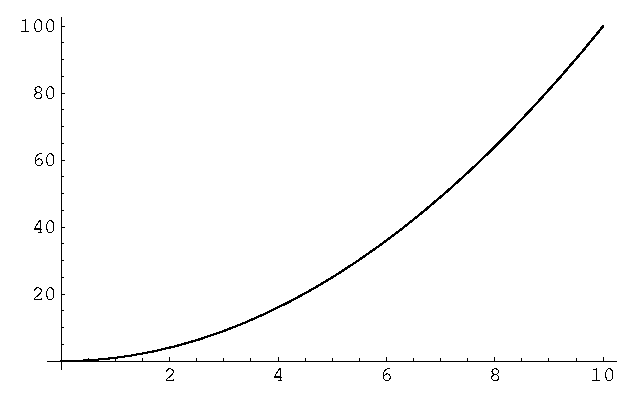
\includegraphics{plot.eps}
  \caption{%
    By default figures are not centered.
    This is a long caption to demonstrate that captions are single spaced.
  }
  \label{fi:not-centered}
\end{figure}

\Repeat{This is the second paragraph.}{10}

\begin{figure}[h]
  \centering
  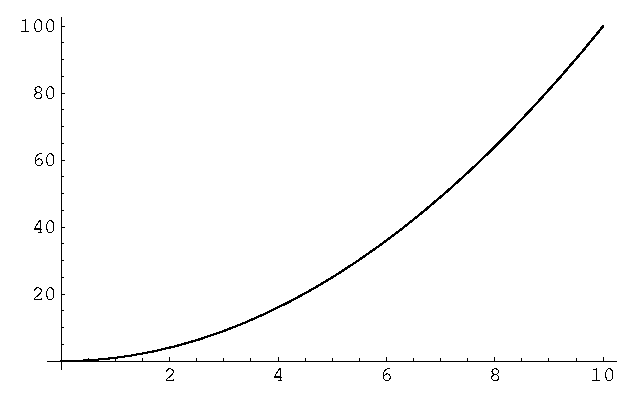
\includegraphics{plot.eps}
  \caption{Use {\tt \char'134centering\/} to center figures.}
  \label{fi:centered}
\end{figure}

\Repeat{This is the third paragraph.}{15}

\begin{figure}[h]
  \centering
  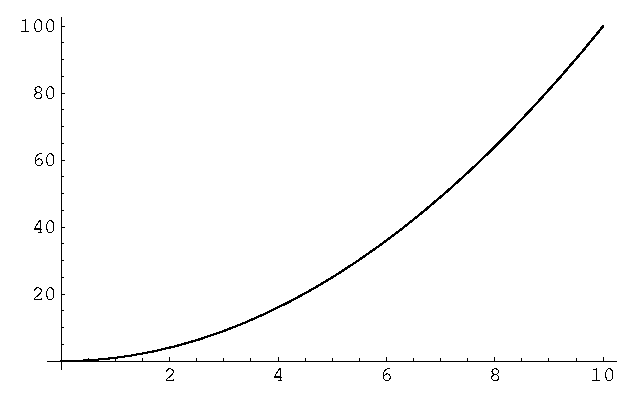
\includegraphics{plot.eps}
  \caption{This is another figuure.}
  \label{fi:another}
\end{figure}

\Repeat{This is the fourth paragraph.}{10}

\begin{figure}[h]
  \centering 
  \subfigure[First subcaption.]{\label{sf:two-parts-a}  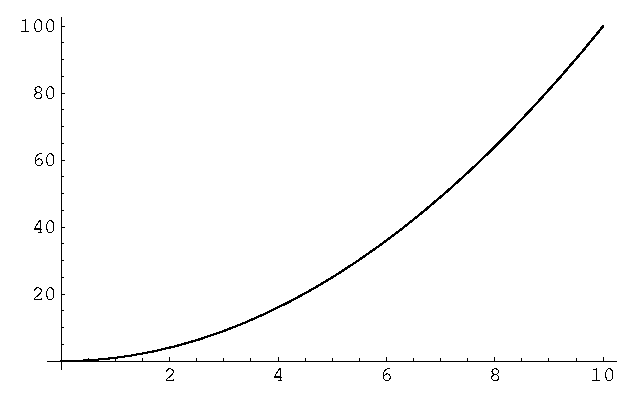
\includegraphics[width=0.3\textwidth]{plot.eps}}%
  \hskip 0.5truein
  \subfigure[Second subcaption.]{\label{sf:two-parts-b}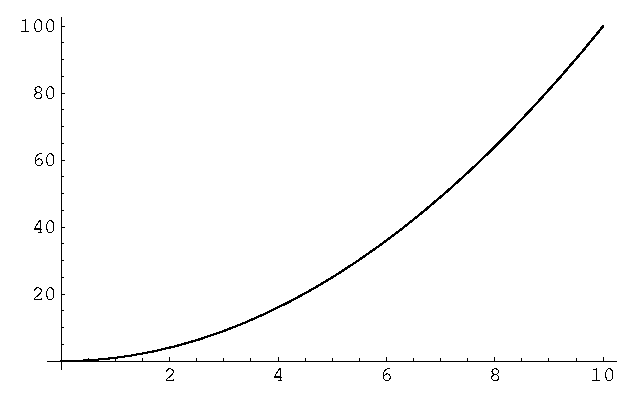
\includegraphics[width=0.3\textwidth]{plot.eps}}
  \caption{This figure has two parts.}
  \label{fi:two-parts}
\end{figure}

\Repeat{This is the fifth paragraph.}{10}

\begin{figure}[h]
  \centering
  \subfigure[First subcaption.]{\label{sf:four-parts-a}  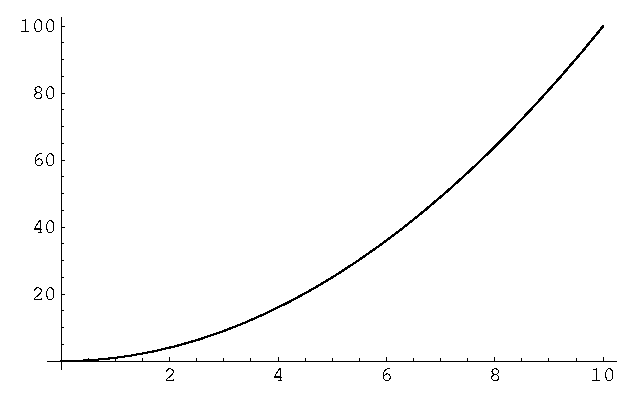
\includegraphics[width=0.3\textwidth]{plot.eps}}%
  \hskip 0.5truein
  \subfigure[Second subcaption.]{\label{sf:four-parts-b}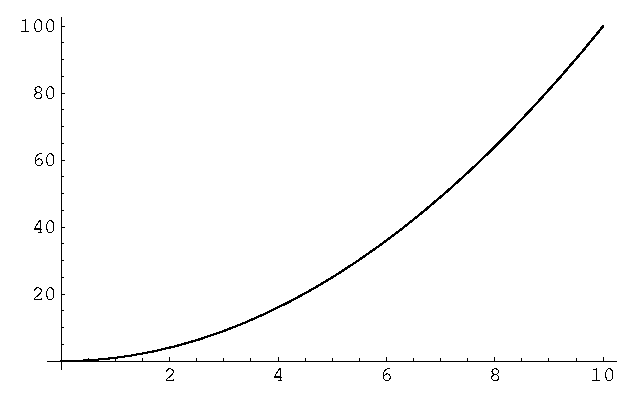
\includegraphics[width=0.3\textwidth]{plot.eps}}
  \subfigure[Third subcaption.]{\label{sf:four-parts-c}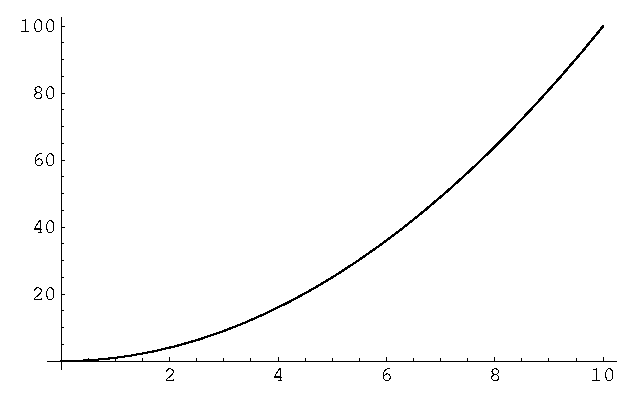
\includegraphics[width=0.3\textwidth]{plot.eps}}%
  \hskip 0.5truein
  \subfigure[Fourth subcaption.]{\label{sf:four-parts-d}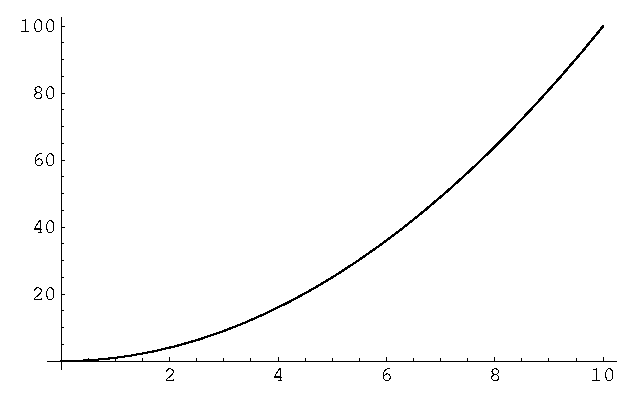
\includegraphics[width=0.3\textwidth]{plot.eps}}
  \caption{This figure has four parts.}
  \label{fi:four-parts}
\end{figure}

\Repeat{This is the sixth paragraph.}{10}

%%
%  THIS FILE DOES SOME UNUSUAL THINGS TO MAKE
%  IT EASIER TO DO DEMONSTRATIONS.  IT SHOULD
%  NOT BE USED AS AN EXAMPLE OF HOW TO PREPARE
%  A FILE.  SEE THE OUTPUT OF THIS FOR LATEX
%  INPUT AND OUTPUT EXAMPLES.
%




%
%  demo-mathematics.tex  2008-12-09  Mark Senn  http://engineering.purdue.edu/~mark
%

\chapter{Demonstrate Mathematics}

    % Use single spacing.
    \Baselinestretch{1}

    % You don't normally need this.
    \mbox{}

    \begin{verbatim}
% From _More Math Into LaTeX_, 4th Edition, page 152:
%     TeX uses $$ to open and close a displayed math environment.
%     In LaTeX, this may occassionally cause problems.  Don't do it.
\[
    E = mc^2
\]
    \end{verbatim}
% From _More Math Into LaTeX_, 4th Edition, page 152:
%     TeX uses $$ to open and close a displayed math environment.
%     In LaTeX, this may occassionally cause problems.  Don't do it.
\[
    E = mc^2
\]
    \vskip\baselineskip
    \hrule
    \vskip0.5\baselineskip
    \filbreak

    \begin{verbatim}
\begin{equation}
    E = mc^2
\end{equation}
    \end{verbatim}
\begin{equation}
    E = mc^2
\end{equation}
    \vskip\baselineskip
    \hrule
    \vskip0.5\baselineskip
    \filbreak

    \begin{verbatim}
% Mydefs.tex defines \be to be \begin{equation} and
% \ee to be \end{equation}.
\be
    E = mc^2
\ee
    \end{verbatim}
% Mydefs.tex defines \be to be \begin{equation} and
% \ee to be \end{equation}.
\be
    E = mc^2
\ee
    \vskip\baselineskip
    \hrule
    \vskip0.5\baselineskip
    \filbreak

    \begin{verbatim}
\be
    x = -\frac{b}{2a} \pm \frac{\sqrt{b^2 - 4ac}}{2a}
\ee
    \end{verbatim}
\be
    x = -\frac{b}{2a} \pm \frac{\sqrt{b^2 - 4ac}}{2a}
\ee
    \vskip\baselineskip
    \hrule
    \vskip0.5\baselineskip
    \filbreak

    \begin{verbatim}
% requires \usepackage{amsmath}; use align* for no equation number
\begin{align}
    a = {}& b + c\\
    x = {}& y + z
\end{align}
    \end{verbatim}
% requires \usepackage{amsmath}; use align* for no equation number
\begin{align}
    a = {}& b + c\\
    x = {}& y + z
\end{align}
    \vskip\baselineskip
    \hrule
    \vskip0.5\baselineskip
    \filbreak

    \begin{verbatim}
\[
    Z = \left(
        \begin{array}{cc}
            a& b\\
            c& d
        \end{array}
    \right)
\]
    \end{verbatim}
\[
    Z = \left(
        \begin{array}{cc}
            a& b\\
            c& d
        \end{array}
    \right)
\]
    \vskip\baselineskip
    \hrule
    \vskip0.5\baselineskip
    \filbreak

    \begin{verbatim}
\begin{equation}
    \begin{split}
        a = {}& b + c\\
            {}& + d + e
    \end{split}      
\end{equation}
    \end{verbatim}
\begin{equation}
    \begin{split}
        a = {}& b + c\\
            {}& + d + e
    \end{split}      
\end{equation}
    \vskip\baselineskip
    \hrule
    \vskip0.5\baselineskip
    \filbreak

    \begin{verbatim}
\be
    (\cos x)^2 + (\sin x)^2 = 1
\ee
    \end{verbatim}
\be
    (\cos x)^2 + (\sin x)^2 = 1
\ee
    \vskip\baselineskip
    \hrule
    \vskip0.5\baselineskip
    \filbreak

    \begin{verbatim}
If $X = \cos x$ and $Y = \sin x$ then $X^2 + Y^2 = 1$.
    \end{verbatim}
If $X = \cos x$ and $Y = \sin x$ then $X^2 + Y^2 = 1$.
    \vskip\baselineskip
    \hrule
    \vskip0.5\baselineskip
    \filbreak

%%
%  demo-multicols.tex  2007-03-19  Mark Senn  http://www.ecn.purdue.edu/~mark
%
%  Demonstrate multicols.
%
%  The multicols package must be loaded for this to work.
%  To load the multicols package put
%      \usepackage{multicols}
%  between the "\documentclass" and "\begin{document}" commands.
%

\chapter{Demonstrate Multicols}

% Put this amount of space between the columns.
\setlength{\columnsep}{0.5truein}

% Separate the columns with a vertical rule this wide.
\setlength{\columnseprule}{0.4pt}

\Repeat{This is one column.}{25}

\begin{multicols}{2}
\Repeat{This is two columns.}{25}
\end{multicols}

\begin{multicols}{3}
\Repeat{This is three columns.}{25}
\end{multicols}

\begin{multicols}{4}
\Repeat{This is four columns.}{25}
\end{multicols}

\begin{multicols}{5}
\Repeat{This is five columns.}{25}
\end{multicols}

%%
%  demo-tables.tex  2014-08-08  Mark Senn
%
%  Demonstrate how to do tables.
%

\chapter{Demonstrate Tables}

% \newlength{\ta}
% \newlength{\tb}
% \newlength{\tc}
% 
% \settowidth{\ta}{\vbox{\hbox{Money}\hbox{Market}}}
% \settowidth{\tb}{\vbox{\hbox{Stocks}\hbox{and}\hbox{Bonds}}}
% \settowidth{\tc}{\vbox{\hbox{Money}\hbox{Market}\hbox{and}\hbox{Stocks}}}
% 
% {
%     \renewcommand{\baselinestretch}{1}
%     \begin{table}
%       \caption{%
%         \hfil Allocation of the IRA and Keogh Wealth\hfil\break
%         \mbox{}\hfil for Investors With or Without Brokerage Accounts\hfil
%       }
%       \label{tab:ira}
%       \begin{center}
%         \begin{tabular}%
%           {%
%             |%
%             c%
%             |%
%             >{\centering\hspace{0pt}}m{\the\ta}%  Money Market
%             |%
%             c%                                    Stocks 
%             |%
%             c%                                    Bonds
%             |%
%             c%                                    Diversified
%             |%
%             >{\centering\hspace{0pt}}m{\the\tb}%  Stocks and Bonds
%             |%
%             >{\centering\hspace{0pt}}m{\the\tc}%  Money Market and Stocks
%             |%
%             c%                                    Others
%             |%
%           }
%           \hline
%           IMP&
%             Money Market&
%             Stocks&
%             Bonds&
%             Diversified&
%             Stocks and Bonds&
%             Money Market and Stocks&
%             Others\tabularnewline
%           \hline
%           1& 14.19\%& 57.71\%& 12.21\%& 4.50\%& 7.36\%& 3.04\%& 0.99\%\tabularnewline \hline
%           2& 14.08\%& 58.18\%& 12.32\%& 4.44\%& 7.30\%& 2.80\%& 0.88\%\tabularnewline \hline
%           3 &14.26\%& 58.09\%& 12.27\%& 4.50\%& 7.19\%& 2.75\%& 0.94\%\tabularnewline \hline
%           4 &13.94\%& 58.11\%& 12.14\%& 4.78\%& 7.35\%& 2.68\%& 0.99\%\tabularnewline \hline
%           5 &13.92\%& 58.13\%& 11.93\%& 4.56\%& 7.60\%& 2.98\%& 0.88\%\tabularnewline \hline
%         \end{tabular}
%       \end{center}
%       This table presents the allocations of the wealth in the IRA
%       and Keogh accounts in various asset classes.
%       Results from each set of imputed data are presented here.
%       The first column lists the number of the imputations,
%       and rest of the columns lists various allocations.
%       Entrees under each asset class show the percentage of investors
%       who have most of their IRA
%       and Keogh wealth invested in that particular asset class.
%       The asset class Diversified
%       includes stocks,
%       bonds,
%       and money market investments.
%       The asset class Others
%       include investments in various life insurance products,
%       annuities,
%       real estate, etc.
%       \medskip
%     \footnotesize SOURCE: Survey of Consumer Finances,
%     2001,
%     Federal Reserve Board,
%     USA.\par
%   \end{table}
% }

Here is a really simple table.

% "h" means put table here---don't let it float to top or bottom of page
\begin{table}[h]
  \caption{American Presidents}
  \begin{center}
    \begin{tabular}{rl}
      \bf Number& \bf Name\\
      1& George Washington\\
      2& John Adams\\
      3& Thomas Jefferson\\
    \end{tabular}
  \end{center}
  \label{ta:American-Presidents}
\end{table}

There are 72.27 points per inch.
I like to put 2 points of vertical space between the heading
(Number Name)
and the first line
(1 George Washington)
of the table.

\begin{table}[h]
  \caption{American Presidents with 2pt vertical space after heading}
  \begin{center}
    \begin{tabular}{rl}
      \bf Number& \bf Name\\[2pt]  % put 2pt vertical space after this line
      1& George Washington\\
      2& John Adams\\
      3& Thomas Jefferson\\
    \end{tabular}
  \end{center}
  \label{ta:American-Presidents-with-2pt}
\end{table}

\LaTeX\ can print horizontal and vertical rules in tables.
I don't like the way this looks.

\begin{table}[h]
  \caption{American Presidents with horizontal and vertical lines}
  \begin{center}
    % "|" prints a vertical rule, "c" means center
    \begin{tabular}{|c|l|}
      % "\hline" prints a horizontal rule
      \hline
      \bf\#& \bf Name\\
      \hline
      1& George Washington\\
      \hline
      2& John Adams\\
      \hline
      3& Thomas Jefferson\\
      \hline
    \end{tabular}
  \end{center}
  \label{ta:American-Presidents-with-horizontal}
\end{table}

\newpage

Here is a more complicated table.

\begin{table}[h]
  \caption{C Bitwise Operators}
  \begin{center}
    % "|" prints a vertical rule, "c" means center
    \begin{tabular}{cccc}
      \bf A& \bf B& \bf A$|$B& \bf A\&B\\[2pt]
      0& 0& 0& 0\\
      0& 1& 1& 0\\
      1& 0& 1& 0\\
      1& 1& 1& 1\\
    \end{tabular}
  \end{center}
  \label{ta:C-Bitwise}
\end{table}

You can use Plain \TeX's \verb+\halign+ command to make tables also.
If you can't do a complicated table using \LaTeX\ commands
you may want to try using Plain \TeX\ commands.
\LaTeX's table making commands use Plain \TeX\ commands.

\begin{table}[h]
  \caption{American Presidents using {\tt\char'134 halign}}
  \hbox to \textwidth{\hss\vbox{\halign{%
    \strut #&      % 0. \strut
    \hfil#\qquad&  % 1. Number
    #\hfil\cr      % 2. Name
    %
    & \bf Number& \bf Name\cr
    \noalign{\vskip 2pt}
    & 1& George Washington\cr
    & 2& John Adams\cr
    & 3& Thomas Jefferson\cr
  }}\hss}
  \label{ta:American-Presidents-using}
\end{table}

The next page shows how to do a table that is too long to fit on one page.

\newpage

% This is loosely based on page 106 of _A Guide to LaTeX_, third edition,
% by Helmut Kopka and Patrick W. Daly.
\begin{longtable}{|l|l|}
    \caption{State Abbreviations}\\
    \hline
    State& Abbreviation\\
    \hline
  \endfirsthead
    \caption[]{\emph{continued}}\\
    \hline
    State& Abbreviation\\
    \hline
  \endhead
    \hline
    \multicolumn{2}{r}{\emph{continued on next page}}
  \endfoot
    \hline
  \endlastfoot
  Alabama& AL\\
  Alaska& AK\\
% American Samoa& AS\\
  Arizona& AZ\\
  Arkansas& AR\\
% Armed Forces Europe& AE\\
% Armed Forces Pacific& AP\\
% Armed Forces the Americas& AA\\
  California& CA\\
  Colorado& CO\\
  Connecticut& CT\\
  Delaware& DE\\
% District of Columbia& DC\\
% Federated States of Micronesia& FM\\
  Florida& FL\\
  Georgia& GA\\
% Guam& GU\\
  Hawaii& HI\\
  Idaho& ID\\
  Illinois& IL\\
  Indiana& IN\\
  Iowa& IA\\
  Kansas& KS\\
  Kentucky& KY\\
  Louisiana& LA\\
  Maine& ME\\
% Marshall Islands& MH\\
  Maryland& MD\\
  Massachusetts& MA\\
  Michigan& MI\\
  Minnesota& MN\\
  Mississippi& MS\\
  Missouri& MO\\
  Montana& MT\\
  Nebraska& NE\\
  Nevada& NV\\
  New Hampshire& NH\\
  New Jersey& NJ\\
  New Mexico& NM\\
  New York& NY\\
  North Carolina& NC\\
  North Dakota& ND\\
% Northern Mariana Islands& MP\\
  Ohio& OH\\
  Oklahoma& OK\\
  Oregon& OR\\
  Pennsylvania& PA\\
% Puerto Rico& PR\\
  Rhode Island& RI\\
  South Carolina& SC\\
  South Dakota& SD\\
  Tennessee& TN\\
  Texas& TX\\
  Utah& UT\\
  Vermont& VT\\
% Virgin Islands& VI\\
  Virginia& VA\\
  Washington& WA\\
  West Virginia& WV\\
  Wisconsin& WI\\
  Wyoming& WY\\
\end{longtable}

\newcommand{\cbackslash}{\char'134}
\newcommand{\copencurly}{\char'173}
\newcommand{\cclosecurly}{\char'175}

\newlength{\twidth}
\newlength{\theight}

\setlength{\twidth}{\textwidth}
\setlength{\theight}{\textheight}

\begin{sidewaystable}
  % The following two lines compensate for what I think is a bug.
  \setlength{\textwidth}{\theight}
  \setlength{\textheight}{\twidth}
  \caption{%
    sidewaystable
    {\tt\cbackslash begin\copencurly tabular\cclosecurly\/}%
    \ldots
    {\tt\cbackslash end\copencurly tabular\cclosecurly\/}%
  }
  \begin{center}
    \begin{tabular}{rl}
      \bf Number& \bf Name\\[2pt]  % put 2pt vertical space after this line
      1& George Washington\\
      2& John Adams\\
      3& Thomas Jefferson\\
    \end{tabular}
  \end{center}
\end{sidewaystable}

\begin{sidewaystable}
  % The following two lines compensate for what I think is a bug.
  \setlength{\textwidth}{\theight}
  \setlength{\textheight}{\twidth}
  \caption{%
    sidewaystable
    {\tt\cbackslash halign\copencurly}\ldots{\tt\cclosecurly\/} table%
  }
  \hbox to \textwidth{\hss\vbox{\halign{%
    \strut #&      % 0. \strut
    \hfil#\qquad&  % 1. Number
    #\hfil\cr      % 2. Name
    %
    & \bf Number& \bf Name\cr
    \noalign{\vskip 2pt}
    & 1& George Washington\cr
    & 2& John Adams\cr
    & 3& Thomas Jefferson\cr
  }}\hss}
\end{sidewaystable}

%\newlength{\ta}
%\settowidth{\ta}{\vbox{\hbox{Money}\hbox{Market}}}
%\newlength{\tb}
%\settowidth{\tb}{\vbox{\hbox{Stocks}\hbox{and}\hbox{Bonds}}}
%\newlength{\tc}
%\settowidth{\tc}{\vbox{\hbox{Money}\hbox{Market}\hbox{and}\hbox{Stocks}}}
%
%  {\renewcommand{\baselinestretch}{1}
%\begin{table}
%  \caption{\hfil Allocation of the IRA and Keogh Wealth\hfil\break\mbox{}\hfil for Investors With or Without Brokerage Accounts\hfil}
%  \label{tab:ira}
%  \begin{center}
%    \begin{tabular}%
%      {%
%        |%
%        c%
%        |%
%        >{\centering\hspace{0pt}}m{\the\ta}%  Money Market
%        |%
%        c%                                    Stocks 
%        |%
%        c%                                    Bonds
%        |%
%        c%                                    Diversified
%        |%
%        >{\centering\hspace{0pt}}m{\the\tb}%  Stocks and Bonds
%        |%
%        >{\centering\hspace{0pt}}m{\the\tc}%  Money Market and Stocks
%        |%
%        c%                                    Others
%        |%
%      }
%      \hline
%      IMP&
%        Money Market&
%        Stocks&
%        Bonds&
%        Diversified&
%        Stocks and Bonds&
%        Money Market and Stocks&
%        Others\tabularnewline
%      \hline
%      1& 14.19\%& 57.71\%& 12.21\%& 4.50\%& 7.36\%& 3.04\%& 0.99\%\tabularnewline \hline
%      2& 14.08\%& 58.18\%& 12.32\%& 4.44\%& 7.30\%& 2.80\%& 0.88\%\tabularnewline \hline
%      3 &14.26\%& 58.09\%& 12.27\%& 4.50\%& 7.19\%& 2.75\%& 0.94\%\tabularnewline \hline
%      4 &13.94\%& 58.11\%& 12.14\%& 4.78\%& 7.35\%& 2.68\%& 0.99\%\tabularnewline \hline
%      5 &13.92\%& 58.13\%& 11.93\%& 4.56\%& 7.60\%& 2.98\%& 0.88\%\tabularnewline \hline
%    \end{tabular}
%  \end{center}
%  This table presents the allocations of the wealth in the IRA
%  and Keogh accounts in various asset classes.
%  Results from each set of imputed data are presented here.
%  The first column lists the number of the imputations,
%  and rest of the columns lists various allocations.
%  Entrees under each asset class show the percentage of investors
%  who have most of their IRA
%  and Keogh wealth invested in that particular asset class.
%  The asset class Diversified
%  includes stocks,
%  bonds,
%  and money market investments.
%  The asset class Others
%  include investments in various life insurance products,
%  annuities,
%  real estate, etc.
%  \medskip
%  \footnotesize SOURCE: Survey of Consumer Finances,
%  2001,
%  Federal Reserve Board,
%  USA.\par
%\end{table}
%  }


%%
%  demo-text.tex  2007-07-17  Mark Senn  http://engineering.purdue.edu/~mark
%

\chapter{Demonstrate Text}

% Use single spacing.
\Baselinestretch{1}

% You don't normally need this.
\mbox{}


%\vbox{
\begin{verbatim}
This is a sentence.
This is a sentence.
This is a sentence.
This is a sentence.
This is a sentence.

This is a sentence.
This is a sentence.
This is a sentence.
This is a sentence.
This is a sentence.
\end{verbatim}
This is a sentence.
This is a sentence.
This is a sentence.
This is a sentence.
This is a sentence.

This is a sentence.
This is a sentence.
This is a sentence.
This is a sentence.
This is a sentence.
\vskip\baselineskip
\hrule
%}
\vskip0.5\baselineskip
\filbreak

%\vbox{
\begin{verbatim}
From \verb+http://www.biblegateway.com/passage/?book_id=1&chapter=1&version=50+:

\begin{quote}
    1 In the beginning God created the heavens and the earth.
    2 The earth was without form,
    and void;
    and darkness was on the face of the deep.
    And the Spirit of God was hovering over the face of the waters.

    3 Then God said,``Let there be light'';
    and there was light.
    4 And God saw the light,
    that it was good;
    and God divided the light from the darkness.
    5 God called the light Day,
    and the darkness He called Night.
    So the evening and the morning were the first day. 
\end{quote}
\end{verbatim}
From \verb+http://www.biblegateway.com/passage/?book_id=1&chapter=1&version=50+:

\begin{quote}
    1 In the beginning God created the heavens and the earth.
    2 The earth was without form,
    and void;
    and darkness was on the face of the deep.
    And the Spirit of God was hovering over the face of the waters.

    3 Then God said,``Let there be light'';
    and there was light.
    4 And God saw the light,
    that it was good;
    and God divided the light from the darkness.
    5 God called the light Day,
    and the darkness He called Night.
    So the evening and the morning were the first day. 
\end{quote}
\vskip\baselineskip
\hrule
%}
\vskip0.5\baselineskip
\filbreak

%\vbox{
\begin{verbatim}
\begin{description}
    \item[apple]
        A red fruit.
    \item[banana]
        A yellow fruit.
        This sentence is to make the entry longer so you can see what happens.
        This sentence is to make the entry longer so you can see what happens.
    \item[cherry]
        A red friut.
\end{description}
\end{verbatim}
\begin{description}
    \item[apple]
        A red fruit.
    \item[banana]
        A yellow fruit.
        This sentence is to make the entry longer so you can see what happens.
        This sentence is to make the entry longer so you can see what happens.
    \item[cherry]
        A red friut.
\end{description}
\vskip\baselineskip
\hrule
%}
\vskip0.5\baselineskip
\filbreak

%\vbox{
\begin{verbatim}
\begin{enumerate}
    \item apple
    \item banana
        This sentence is to make the entry longer so you can see what happens.
        This sentence is to make the entry longer so you can see what happens.
    \item cherry
\end{enumerate}
\end{verbatim}
\begin{enumerate}
    \item apple
    \item banana
        This sentence is to make the entry longer so you can see what happens.
        This sentence is to make the entry longer so you can see what happens.
    \item cherry
\end{enumerate}
\vskip\baselineskip
\hrule
%}
\vskip0.5\baselineskip
\filbreak


%\vbox{
\begin{verbatim}
\begin{itemize}
    \item apple
    \item banana
        This sentence is to make the entry longer so you can see what happens.
        This sentence is to make the entry longer so you can see what happens.
    \item cherry
\end{itemize}
\end{verbatim}
\begin{itemize}
    \item apple
    \item banana
        This sentence is to make the entry longer so you can see what happens.
        This sentence is to make the entry longer so you can see what happens.
    \item cherry
\end{itemize}
\vskip\baselineskip
\hrule
%}
\vskip0.5\baselineskip
\filbreak

%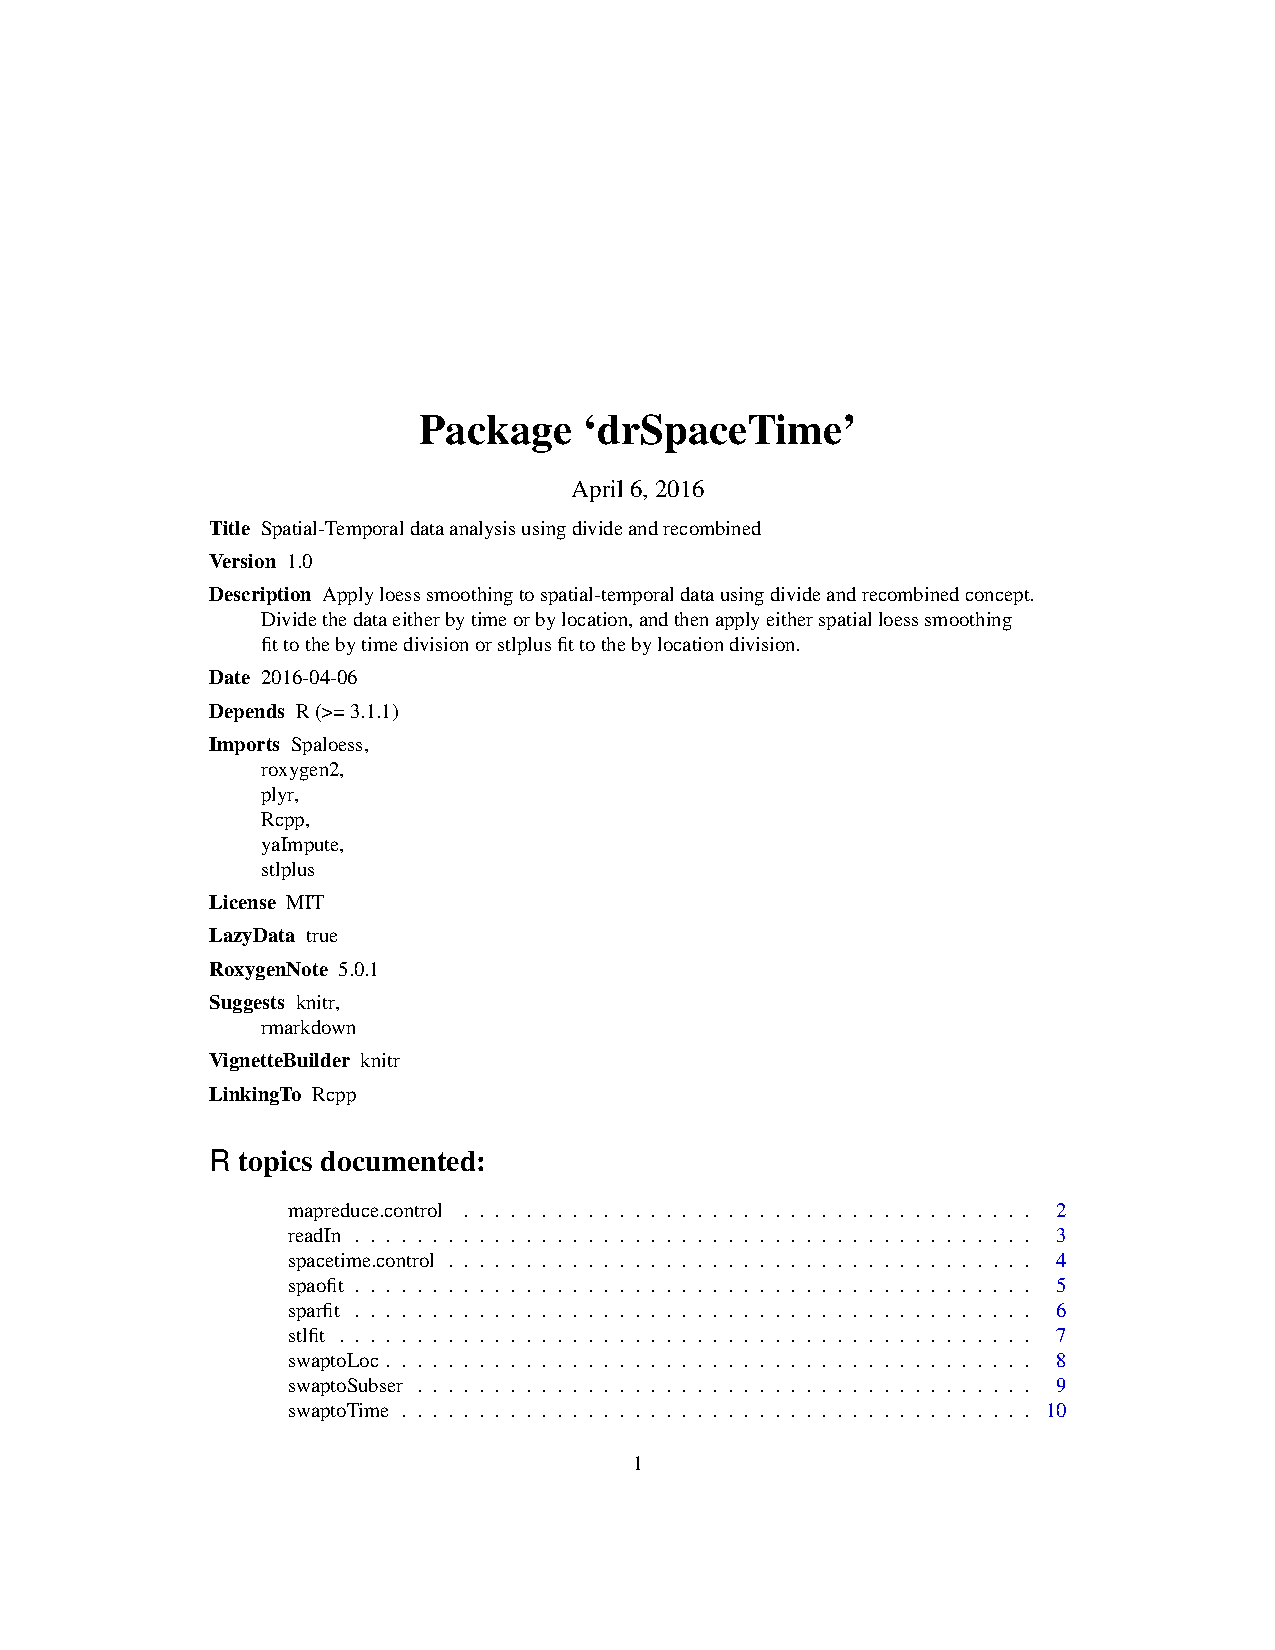
\includepdf[pages={-}]{drSpaceTime.pdf}

%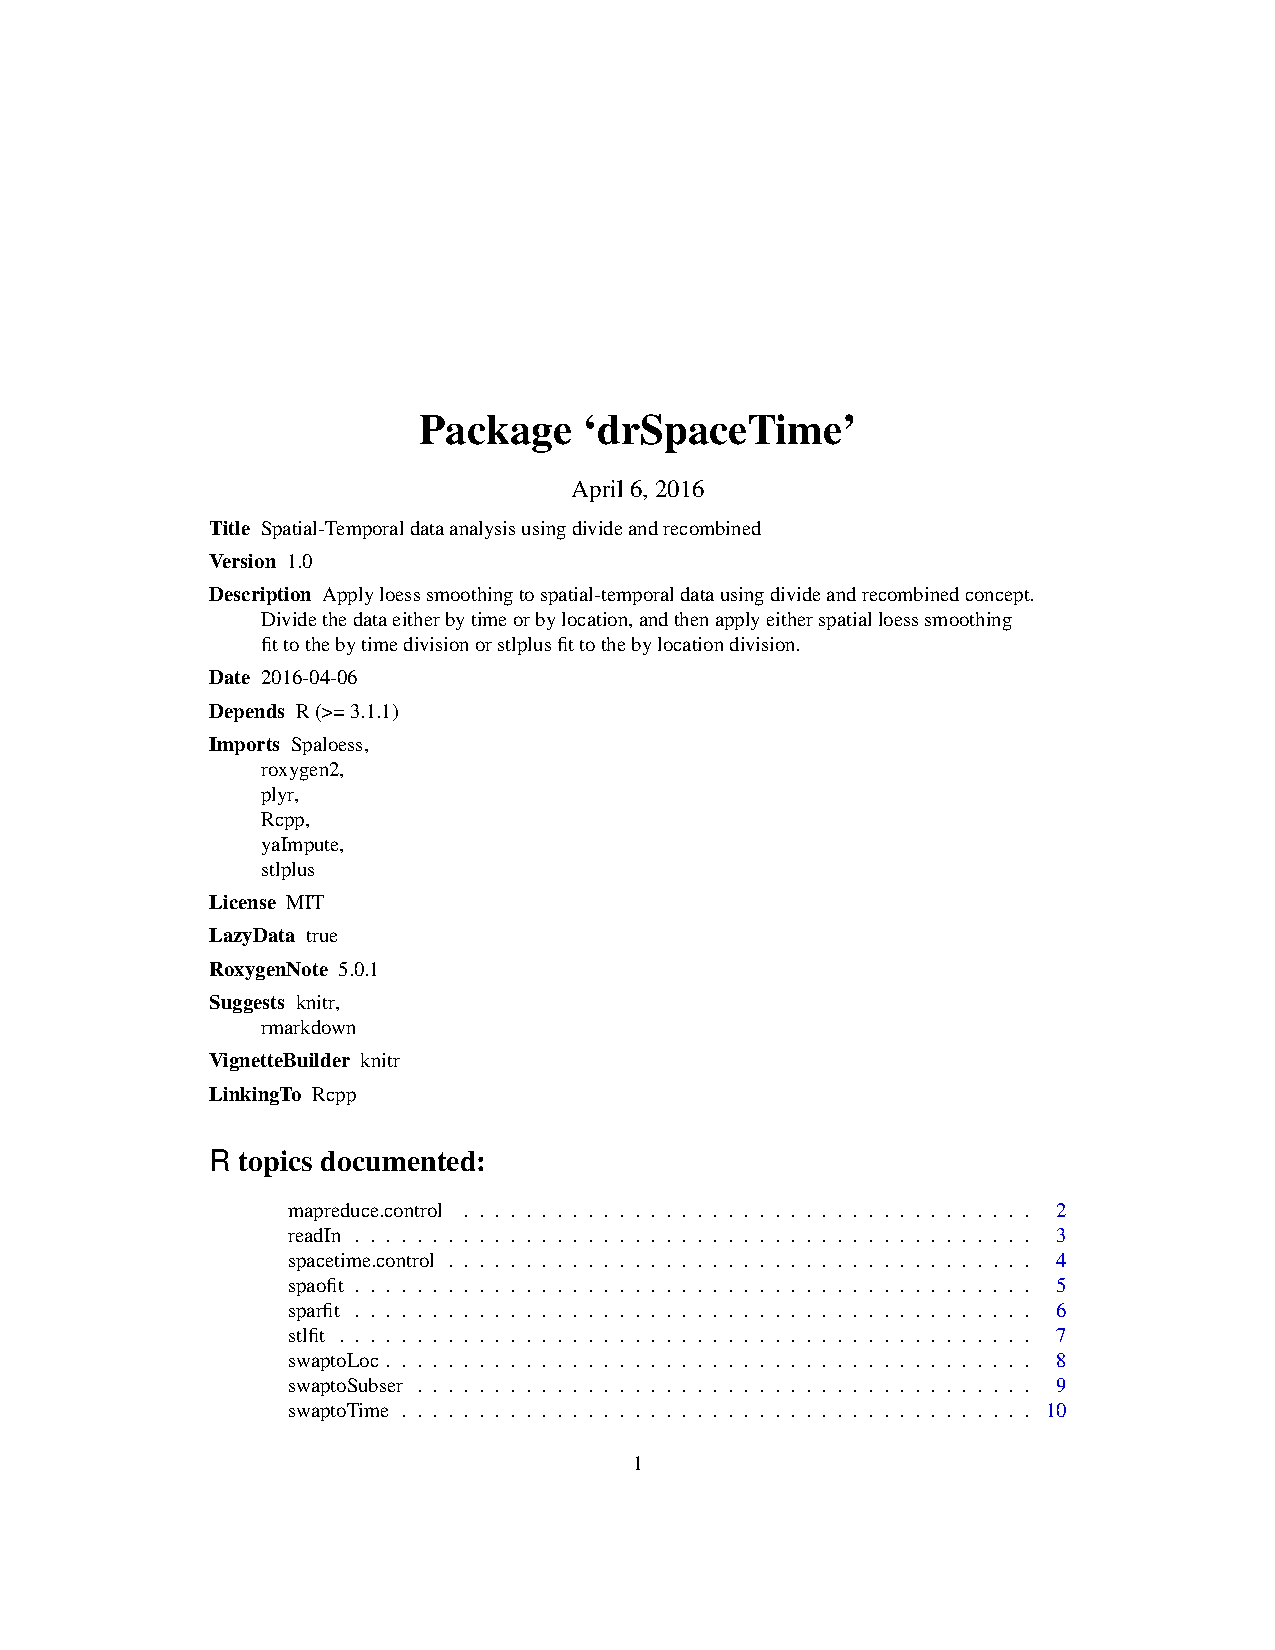
\includepdf[pages=-,scale=.8,pagecommand={}]{drSpaceTime}



\fancypage{\fboxrule=0.5pt\fboxsep=1mm\fbox}{}

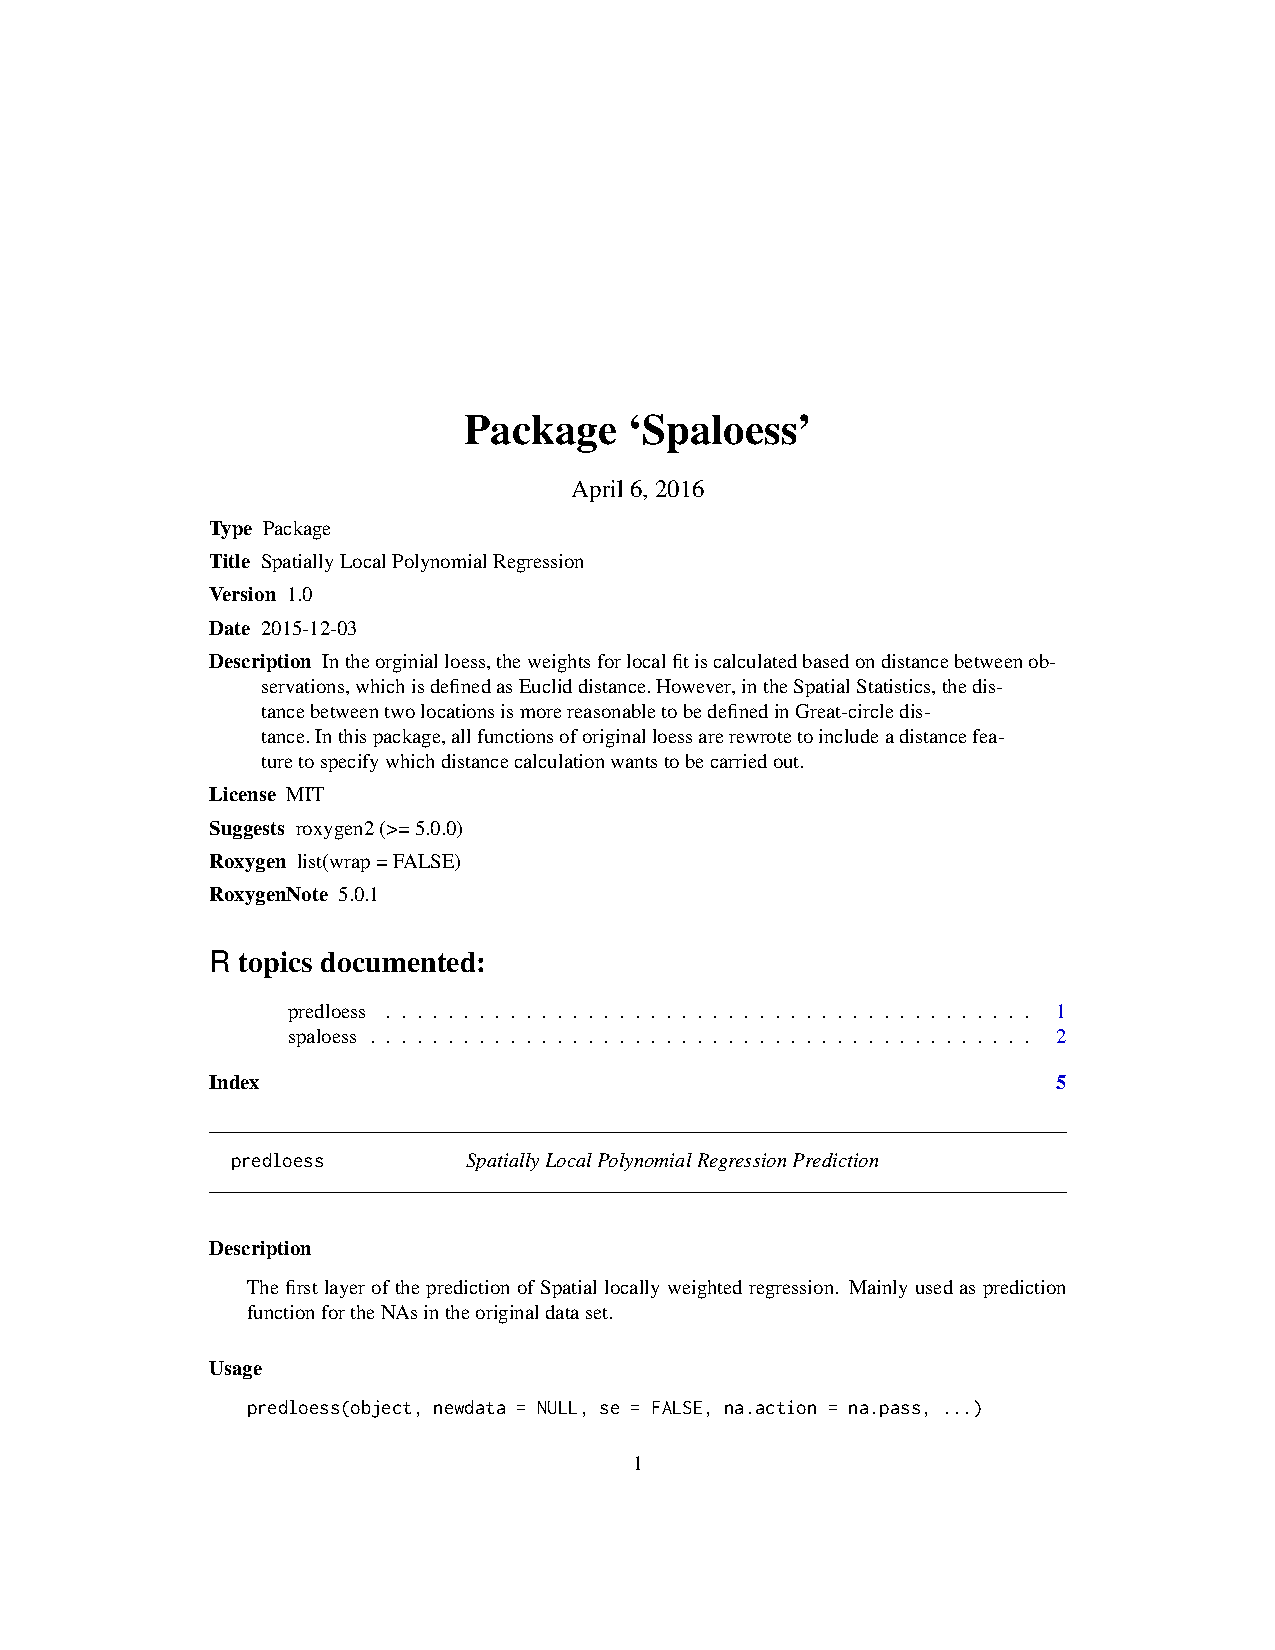
\includepdf[pages=-, pagecommand={},scale=1]{Spaloess.pdf}
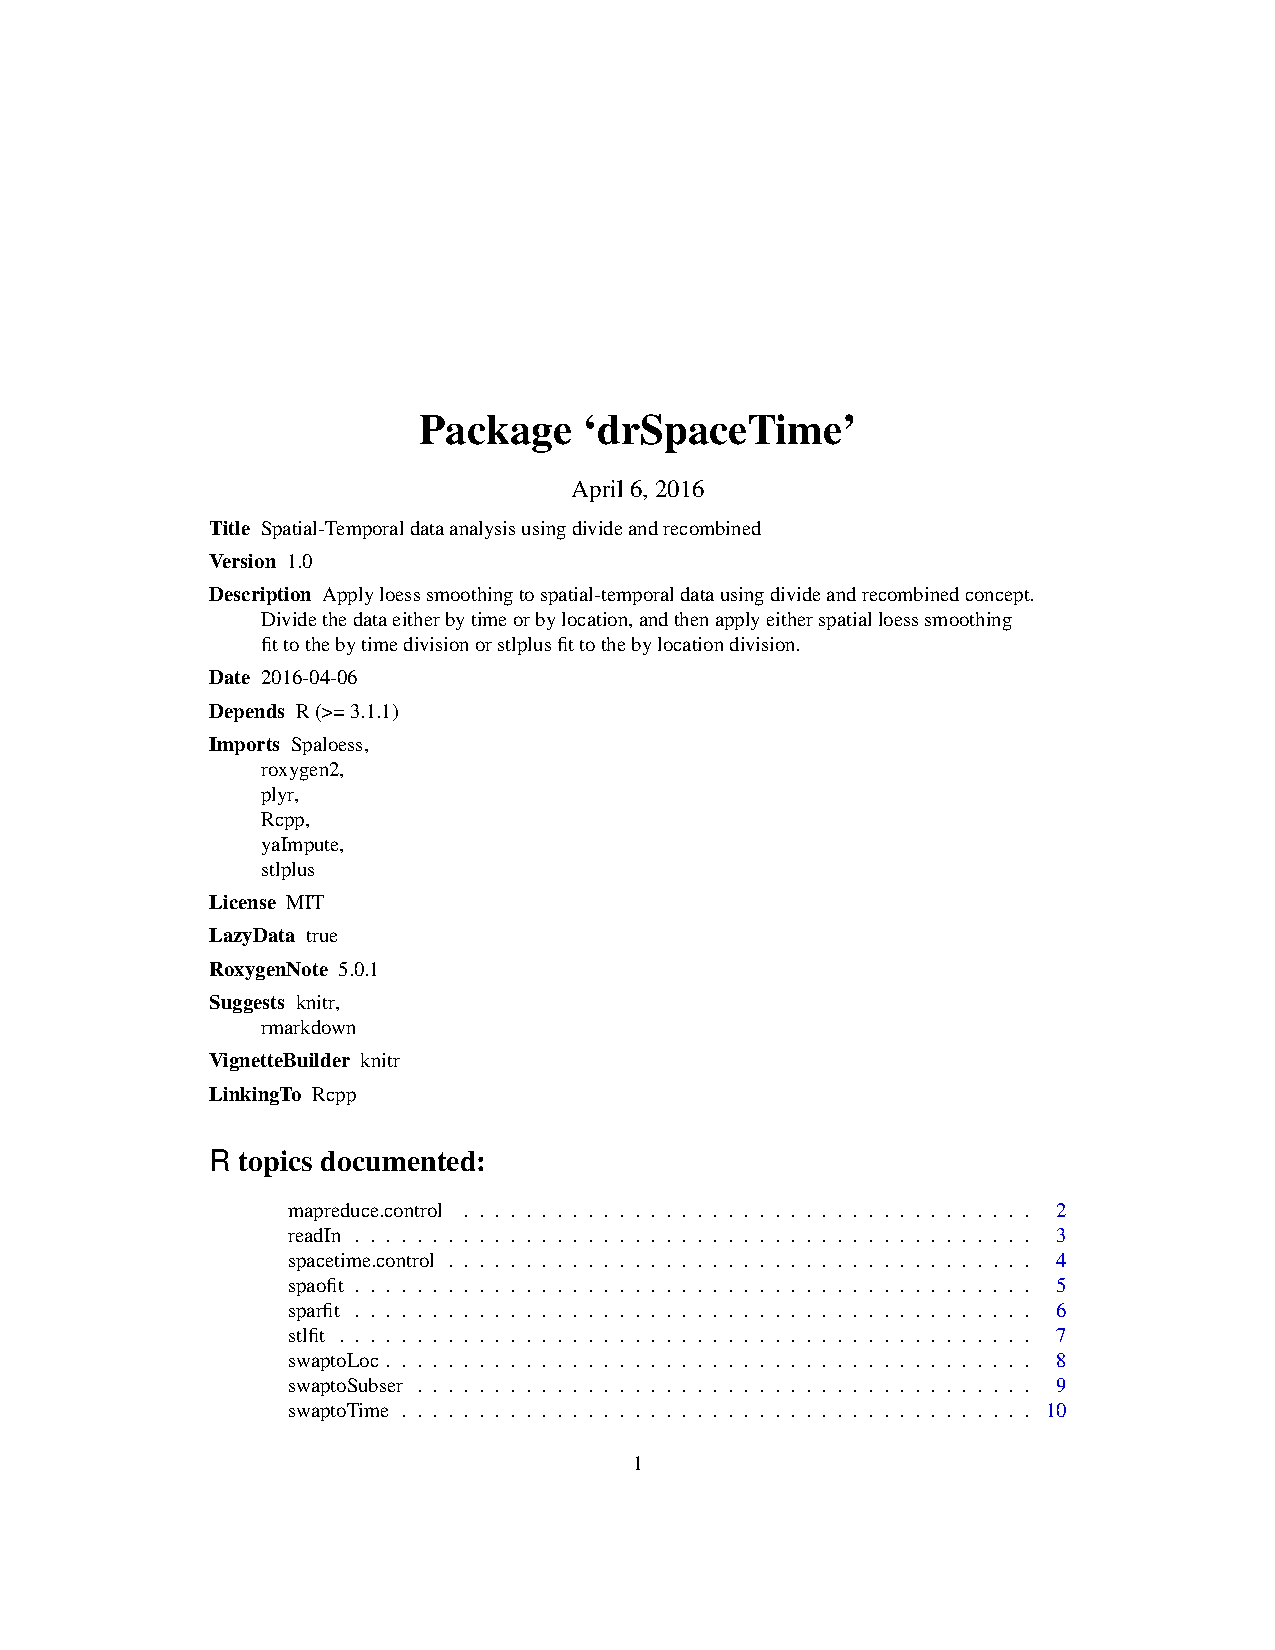
\includepdf[pages=-, pagecommand={},scale=1]{drSpaceTime.pdf}


% Notes and footnotes are optional.
% Reference: TM2006 page 34.
% I have not implemented this yet.  Mark Senn 2002-06-03
%%\include{notes}

% A vita is optional for masters theses
% and required for doctoral dissertations.
% Reference: TM2006 page 13.
% CHANGE NEXT LINE?
%
%  vita.tex   2003.07.23  14:59:33   Mark Senn <mds@purdue.edu>
%
%  This is the vita for a simple, example thesis.
%
%  A vita is required only in a doctoral dissertation.
%

\begin{vita}

Xiaosu Tong was born in Xichang, Sichuan, China in 1988. He earned his B.S. in 
Information and Calculation Science at College of Science, Shenyangjianzhu 
University, China in 2010. Then he pursued his M.S. in Applied Statistics at Purdue
University, Indiana in 2012. His academic interests include exploratory data 
analysis, data visualization, time series, and statistical computation with
large and complex data.

\end{vita}


\end{document}

% LaTeX won't read after the \end{document} command.
% You can put notes to yourself or LaTeX input not
% ready for use here if you'd like.
